\documentclass[conference,10pt]{IEEEtran}
% Note: To compile in clean single-column format for Overleaf or arXiv review, replace line 1 with:
% \documentclass[conference,onecolumn,11pt]{IEEEtran}

\usepackage{cite}
\usepackage{amsmath,amssymb,amsfonts,amsthm}
\usepackage{algorithmic}
\usepackage{graphicx}
\usepackage{textcomp}
\usepackage{xcolor}
\usepackage{booktabs}
\usepackage{array}
\usepackage{silence}
\WarningFilter{latex}{Command \showhyphens}
\usepackage{microtype}
\usepackage{url}
\usepackage{hyperref}
\usepackage{tikz}
\usetikzlibrary{shapes.geometric, arrows.meta, positioning, calc}

\newtheorem{definition}{Definition}
\newtheorem{theorem}{Theorem}
\newtheorem{lemma}{Lemma}

\definecolor{googleblue}{HTML}{1A73E8}
\definecolor{googlegreen}{HTML}{1E8E3E}
\definecolor{googlered}{HTML}{D93025}

\hypersetup{
    colorlinks=true,
    linkcolor=googleblue,
    citecolor=googleblue,
    urlcolor=googleblue
}

\begin{document}

\title{Agent-Notary: Cryptographic Non-Repudiation, Zero-Knowledge Invariant Attestation, and Merkle-DAG Action Provenance for Autonomous Multi-Agent Swarms}

\author{
\IEEEauthorblockN{Aniket Agrawal}
\IEEEauthorblockA{Cloud Engineer, Google Cloud \\
Google, Bangalore, India \\
aniketagrawal@google.com}
}

\maketitle

\begin{abstract}
As enterprise computing systems adopt multi-agent workflows---coordinated across platforms such as Google Cloud Vertex AI Agent Builder and the Model Context Protocol (MCP)---agents increasingly execute state-mutating operations across external databases, financial settlement APIs, and cloud infrastructure. However, existing agent orchestration runtimes lack cryptographic action provenance and non-repudiation across service boundaries. When a sub-agent executes a tool invocation induced by an indirect prompt injection or reasoning error, standard telemetry systems (e.g., OpenTelemetry, cloud audit trails) record only mutable, unauthenticated textual logs that can be modified, repudiated, or omitted by compromised components. Furthermore, enterprise compliance requires cryptographic verification that policy invariants were satisfied without exposing sensitive customer context or raw prompt tokens to external auditors.

In this paper, we present \textbf{Agent-Notary}, a low-latency cryptographic attestation and non-repudiation framework for distributed multi-agent workflows. Agent-Notary introduces three core mechanisms: (1) an append-only \textbf{Causal Merkle-DAG} that binds multi-agent request and completion vertices ($v_i^{\text{req}} \to v_i^{\text{resp}}$), tool calls, and Lamport timestamps into an immutable cryptographic chain of custody without retroactive digest mutation; (2) a \textbf{Dual-Tier Blinded Policy-Invariant Attestation Engine} that pairs microsecond intra-cluster HKDF-blinded enclave witness tokens on the hot path with hardware-attested Confidential VM commitment equivalence and asynchronous Ristretto255 Pedersen commitments with Fiat-Shamir Bulletproof range/predicate transcripts for third-party public auditability without disclosing sensitive parameters; and (3) a wire-level \textbf{Zero-Knowledge Action Attestation Voucher (ZKA-Voucher)} encapsulated into standard HTTP/2 and gRPC transport metadata headers. Agent-Notary implements a dual-mode cryptographic trust model: service-bound symmetric HMAC authenticators for microsecond intra-cluster tool server verification alongside asymmetric Ed25519 signatures on Merkle frontier epoch roots for third-party public non-repudiation. Empirical evaluation over $N = 1{,}000$ wire/replay tamper traces and $N = 300$ multi-agent indirect prompt-injection traces (modeled on AgentDojo, InjecAgent, and ASB) demonstrates $100.00\%$ detection of wire tampering, signature forgery, replay desynchronization, and out-of-policy prompt injections ($\Pi(t_i, \theta_i) = 0$), $100.00\%$ ($100/100$) post-hoc cryptographic parent-slice attribution of in-policy semantic hijacking ($1.84\,\mu\text{s}$ DAG traversal isolating $82\%$ [$82/82$] context-isolated traces structurally to a single parent, and narrowing the $18\%$ [$18/18$] merged-turn subset to the exact $k_p$-element authenticated parent slice, within which heuristic AST matching pinpoints un-obfuscated parent blobs in $+14.2\,\mu\text{s}$), a line-rate mean intra-cluster verification latency of $4.17\,\mu\text{s}$ (P50: $2.29\,\mu\text{s}$, P95: $11.46\,\mu\text{s}$, P99: $21.96\,\mu\text{s}$), and a compact wire header footprint of $2{,}250\,\text{bytes}$.
\end{abstract}

\begin{IEEEkeywords}
Multi-Agent Systems, Non-Repudiation, Zero-Knowledge Proofs, Merkle DAG, Model Context Protocol, Cryptographic Audit, Cloud Security.
\end{IEEEkeywords}

\section{Introduction}
Large Language Model (LLM) agents are increasingly deployed as distributed multi-agent workflows that interact directly with enterprise backends~\cite{brown2020language, achiam2023gpt4, team2023gemini}. Within enterprise platforms like Vertex AI Agent Builder and the open Model Context Protocol (MCP)~\cite{mcp2024spec}, agent workflows coordinate multi-step operations including enterprise resource planning (ERP) reconciliations, cloud infrastructure provisioning, and financial disbursements.

However, enterprise multi-agent deployments lack end-to-end cryptographic provenance and non-repudiation across delegation hops~\cite{greshake2023not, debenedetti2024agentdojo, zhan2024injecagent}. In a multi-turn workflow, Agent $A$ (e.g., an external customer service intake agent) may ingest an adversarial ticket containing an indirect prompt injection. That injection induces Agent $A$ to issue a compromised task delegation to Agent $B$ (e.g., a privileged financial payment agent), which in turn executes a high-value disbursement API call. When forensic auditors inspect the incident post-hoc, existing telemetry frameworks such as OpenTelemetry and centralized database audit tables provide only mutable, unstructured JSON text logs. These logs exhibit three security limitations:
\begin{enumerate}
    \item \textbf{Vulnerability to Repudiation and Forgery:} Standard API logs lack cryptographic signatures tied to causal execution states. A rogue internal service or an attacker with administrative cloud access can forge, modify, or delete log entries without detection.
    \item \textbf{Causal Disconnection in Heterogeneous Swarms:} When agents operate across organizational or tenant boundaries, asynchronous tool calls become causally untraceable. Standard tracing spans cannot cryptographically prove which upstream agent instruction induced a downstream mutation.
    \item \textbf{Auditability Under Confidentiality Constraints:} Regulatory bodies (e.g., SOX, HIPAA, GDPR) require verification that agent tool invocations adhered to enterprise policy invariants (e.g., transaction limits, sanitized destination buckets). However, providing raw audit logs to external auditors exposes proprietary system prompts, model reasoning chains, and confidential customer PII~\cite{goldwasser1989knowledge}.
\end{enumerate}

To overcome these challenges, this paper presents \textbf{Agent-Notary}, a line-rate cryptographic non-repudiation framework designed for enterprise multi-agent tool execution. Importantly, Agent-Notary establishes a \emph{two-pronged defense posture} (pre-execution enforcement and post-hoc provenance) under an explicit \textbf{Trusted Computing Base (TCB)}: the out-of-process Agent-Notary Gateway sidecar and the host orchestration harness's deterministic sub-session context-propagation multiplexer execute co-resident inside the calling agent's hardware-attested Confidential VM enclave boundary (backed by AMD SEV-SNP memory encryption), while destination tool-server verifiers execute inside their respective remote attested enclave boundaries across untrusted network links alongside administrator-provisioned declarative policy circuits $\Pi$. Conversely, LLM reasoning models, host OS/hypervisor/network/logging administrators outside the Confidential VMs, inter-agent network links, local observability databases, and external third-party auditors are strictly untrusted; Google Cloud KMS key release is cryptographically gated by SEV-SNP attestation quotes ($\mathcal{Q}_{\text{TEE}}$), Cloud Spanner/Storage epoch audit anchors enforce WORM retention locks (and replicate $\Sigma_{\text{root}}$ to an external auditor domain), and the gateway journals tool responses to a write-once AES-256-GCM encrypted payload escrow store. Specifically, a per-epoch root escrow secret $\text{sk}_{\text{escrow}}$ is wrapped once per epoch under the KMS-attested auditor public key, and each vertex derives a single-use key $k_{\text{escrow},k} = \operatorname{HKDF-SHA256}(\text{sk}_{\text{escrow}}, \mathtt{0x11} \parallel \mathtt{0x01} \parallel H(v_k^{\text{resp}}))$ and deterministic 96-bit ($12$-octet) initialization vector $\text{IV}_k = \operatorname{HKDF-Expand}_{96}(\operatorname{HKDF-Extract}(\text{salt}_{\text{notary}}, \text{sk}_{\text{escrow}}), \mathtt{0x11} \parallel \mathtt{0x02} \parallel H(v_k^{\text{resp}}))$---where, as formalized in Section~IV-A, two-argument $\operatorname{HKDF-SHA256}(\text{ikm}, \text{info})$ shorthand expands from the same extracted pseudorandom key $\text{PRK}_{\text{escrow}} = \operatorname{HKDF-Extract}(\text{salt}_{\text{notary}}, \text{sk}_{\text{escrow}})$ so the auditor unwraps $\text{sk}_{\text{escrow}}$ once per epoch and derives $(k_{\text{escrow},k}, \text{IV}_k)$ in memory without per-vertex asymmetric overhead---to encrypt the deterministic RFC 8785 canonical byte buffer $\operatorname{CanonicalJSON}(o_k)$ under AES-256-GCM with $H(v_k^{\text{resp}})$ bound as the Additional Authenticated Data (AAD), guaranteeing deterministic ciphertext idempotency across write retries and immediate AEAD tag rejection if an adversary substitutes ciphertexts across vertices. Crucially, in the single-parent regime ($|\mathcal{P}_i^{\text{req}}| = 1$, $82\%$ of traces), the enclave-resident harness multiplexer spawns per-branch context-isolated LLM sub-invocations whose outbound transport channels are bound to transport-layer session handles mapped to $v_k^{\text{resp}}$ (without relying on the untrusted LLM to echo proxy tokens), whereas multi-parent context merging ($|\mathcal{P}_i^{\text{req}}| = k_p > 1$, $18\%$ of traces) is governed strictly by deterministic join barriers in the trusted harness workflow graph. If a privileged cloud administrator attempts to suppress or truncate already-anchored gateway frames from audit storage, monotonic epoch sequence counters ($\text{seq}_{\text{epoch}}$) and causal parent links in anchored frontier roots expose the omission immediately; while non-escrowed ($\texttt{escrow\_mode} = 0$) calls trade off a bounded $\Delta_{\text{epoch}} = 100\,\text{ms}$ pre-anchoring window for sub-$5\,\mu\text{s}$ dispatch, production deployments enforce a deterministic three-tier policy matrix mapping (i)~read-only/idempotent queries to single-node $\texttt{escrow\_mode} = 0$ ($28.45\,\mu\text{s}$, where the destination verifier's append-only receipt log still records $\mathcal{V}_{\text{wire}}$), (ii)~intermediate-risk reversible mutations to $\texttt{escrow\_mode} = 0$ paired with synchronous multi-replica Redis/\texttt{WAIT 1} and regional Persistent Disk journaling ($213.45\,\mu\text{s}$, eliminating single-host crash loss prior to the $100\,\text{ms}$ tick), and (iii)~high-value or irreversible external mutations to $\texttt{escrow\_mode} = 1$ ($58.40\,\text{ms}$) so destination verifiers hold execution in provisional escrow until Spanner epoch anchoring completes. Conversely, if an unnotarized request is dropped before reaching the gateway sidecar, no ZKA-Voucher is minted and the destination verifier fails closed; if a notarized request ($\mathcal{V}_{\text{wire}}$) is dropped in transit before reaching the destination tool server or if the returning completion frame ($o_i$) is dropped after tool execution, the pre-execution vertex $v_i^{\text{req}}$ ($H_{\text{pending}}$) remains permanently anchored in $R_T$ as an unclosed invocation, and the destination verifier's append-only execution receipt log indexed by $(H_{\text{leaf}}, \text{vid})$ resolves retries idempotently: each destination verifier authenticates execution/error receipts ($\mathtt{0x09} \parallel \mathtt{0x01} \parallel H_{\text{leaf}} \parallel \operatorname{lp}(\text{vid}) \parallel H_{\text{out}}(v_i^{\text{resp}}) \parallel \operatorname{encode}_8(\text{status}) \parallel \operatorname{encode}_{64}(\tau_{\text{ver}})$) and \texttt{NOT\_SEEN} status inquiry receipts ($\mathtt{0x09} \parallel \mathtt{0x02} \parallel H_{\text{leaf}} \parallel \operatorname{lp}(\text{vid}) \parallel \text{``NOT\_SEEN''} \parallel \operatorname{encode}_{64}(\tau_{\text{ver}})$) using its enclave Ed25519 signing key $\text{sk}_{\text{verifier}, t_i}$ (whose public key $\text{pk}_{\text{verifier}, t_i}$ is bound in the verifier's SEV-SNP attestation quote $\mathcal{Q}_{\text{TEE}}$ for third-party public audit verification without $K_{\text{tool}, t_i}$, paired with intra-cluster $\operatorname{HMAC-SHA256}_{K_{\text{tool}, t_i}}$ for microsecond gateway checks). Upon a transport timeout, the gateway always replays the original $\mathcal{V}_{\text{wire}}$ carrying $(H_{\text{leaf}}, \text{vid})$ first---if the initial request executed before the response $o_i$ was dropped, the verifier's Step~2 replay check looks up $(H_{\text{leaf}}, \text{vid})$ in the receipt log and returns the cached signed execution receipt and output $o_i$ idempotently without re-executing $t_i$, whereas if the initial frame never reached the verifier (or only after an explicit $\text{sk}_{\text{verifier}, t_i}$-signed $\mathtt{0x09} \parallel \mathtt{0x02}$ \texttt{NOT\_SEEN} status inquiry), the replayed $\mathcal{V}_{\text{wire}}$ executes normally (or a fresh retry vertex $\textsf{vid}'$ explicitly links to the unclosed $v_i^{\text{req}}$). Under this threat model, Agent-Notary enforces: (i) \emph{pre-execution line-rate enforcement}, deterministically blocking tool invocations whose parameters violate policy invariants ($\Pi(t_i, \theta_i) = 0$) or exhibit wire tampering, forgery, or replay; and (ii) \emph{post-hoc non-repudiable causal provenance}, anchoring multi-agent delegation chains in an append-only Causal Merkle-DAG so that in-policy semantic prompt injections ($\Pi(t_i, \theta_i) = 1$) remain forensically attributable across organizational boundaries without repudiation via the \textbf{Zero-Knowledge Action Attestation Voucher (ZKA-Voucher)}.

\section{Related Work}
\subsection{Multi-Agent Systems, Request Signing, and Privilege Control}
The emergence of standardized tool invocation protocols and benchmarks---most notably the Model Context Protocol (MCP)~\cite{mcp2024spec}, functional suites such as MCP-Universe~\cite{luo2025mcpuniverse} and MCP-Bench~\cite{wang2025mcpbench}, and dedicated MCP security benchmarks including MCPSecBench~\cite{yang2025mcpsecbench}, MCPTox~\cite{wang2025mcptox}, and MCP-SafetyBench~\cite{zong2025mcpsafetybench}---alongside HTTP Message Signatures (RFC 9421)~\cite{backman2024rfc9421}, OAuth 2.0 Token Exchange (RFC 8693)~\cite{jones2020rfc8693}, Demonstrating Proof-of-Possession (DPoP, RFC 9449)~\cite{fett2023dpop}, and attenuated capability token architectures such as Macaroons~\cite{birgisson2014macaroons} and public-key attenuated Eclipse Biscuit tokens~\cite{couprie2025biscuit}, has advanced how distributed services authenticate remote operations. Recent agent identity and governance architectures such as BAID~\cite{lin2025baid}, AIP~\cite{prakash2026aip}, SAGA~\cite{syros2025saga}, and workflow-bound Agentic JWT (A-JWT) delegation extensions over RFC 7519/8693/9449~\cite{jones2015json, jones2020rfc8693, fett2023dpop, goswami2025ajwt} further introduce cryptographic agent identifiers, lifecycle access-control gateways, and session tokens across MCP and A2A boundaries. However, existing authentication and capability frameworks treat authorization predominantly as a session-level handshake or linear delegation chain~\cite{harding2012oauth}. Once an agent establishes an authenticated session, the runtime often retains broad authority across concurrent branches~\cite{saltzer1975protection, zhang2025asb}. While Macaroons provide chained HMAC caveats, Eclipse Biscuit~\cite{couprie2025biscuit}, AIP~\cite{prakash2026aip}, SAGA~\cite{syros2025saga}, and A-JWT~\cite{goswami2025ajwt} add public-key attenuation, governance registries, or workflow token claims, and RFC 9421 / DPoP specify per-request HTTP signing, none bind non-linear branching two-phase causal dependency DAGs ($v_i^{\text{req}} \to v_i^{\text{resp}}$) across asynchronous multi-agent swarms nor provide zero-knowledge policy-invariant attestations over blinded tool arguments.

Concurrently, recent agent-layer security and trace-verification frameworks---including CaMeL~\cite{debenedetti2025camel}, FIDES~\cite{costa2025fides}, Progent~\cite{shi2025progent}, and Verifiable Execution Traces (VET)~\cite{grigor2025vet}---enforce pre-execution data-flow isolation, capability labels, deterministic tool policies, or step-level execution trace signatures. While CaMeL, FIDES, and Progent effectively restrict unauthorized tool calls within a single trusted runtime and VET signs linear step traces, they do not generate sub-$5\,\mu\text{s}$ service-scoped wire vouchers, non-repudiable cross-domain two-phase Merkle-DAG frontier anchors with WORM payload escrow, or Dual-Tier Ristretto255 Bulletproof R1CS parameter proofs verifiable by external third-party auditors when logs are contested or local telemetry is compromised. Agent-Notary is directly complementary to intra-agent IFC/policy engines, providing the cryptographic transport and non-repudiation layer across distributed multi-agent boundaries.

\subsection{Cryptographic Provenance and Transparency Systems}
Cryptographic transparency and supply-chain provenance systems have proven effective in securing distributed infrastructure, most prominently Certificate Transparency (RFC 6962)~\cite{laurie2014certificate}, software supply-chain layout attestation in \textit{in-toto}~\cite{torres2019intoto}, and content-addressed Merkle-CRDTs~\cite{sanjuan2020merkle}. RFC 6962 employs append-only Merkle trees with domain-separated leaf and interior prefixes to detect unauthorized TLS certificate issuance, \textit{in-toto} verifies signed multi-step software pipeline layouts, and Merkle-CRDTs embed causal DAG history into self-verifying conflict-free replicated data types. Similarly, recent W3C PROV-based agentic provenance trackers such as PROV-AGENT~\cite{souza2025provagent} capture semantic causal graphs across MCP tool executions, while emerging COSE-based supply-chain transparency standards such as IETF SCITT~\cite{birkholz2026scitt} (building on RFC 6962~\cite{laurie2014certificate}) issue signed Merkle inclusion receipts over registered artifacts. However, W3C PROV-AGENT graphs are unauthenticated telemetry records lacking cryptographic non-repudiation or zero-knowledge privacy; classical transparency logs and IETF SCITT receipts target linear artifact registration with asymmetric COSE verification rather than sub-$5\,\mu\text{s}$ branching multi-agent RPC streams; \textit{in-toto} targets static build pipelines; and Merkle-CRDTs optimize for eventual-consistency state replication rather than synchronous two-phase request-completion causality ($v_i^{\text{req}} \to v_i^{\text{resp}}$) with blinded zero-knowledge policy-invariant proofs~\cite{lamport1978time}.

\subsection{Zero-Knowledge and Blinded Policy Attestation}
Zero-Knowledge Proofs (ZKPs) allow a prover to convince a verifier that an assertion is mathematically true without disclosing the underlying witness data~\cite{goldwasser1989knowledge, ben2018scalable}. While general-purpose zk-SNARKs and zk-STARKs have been explored for verifiable off-chain computation~\cite{sasson2014zerocash}, recent MCP auditing proposals such as zk-MCP~\cite{jing2025zkmcp} apply zero-knowledge circuit proofs to agent communication logs, and Bulletproofs~\cite{bunz2018bulletproofs} provide short non-interactive range proofs over Pedersen commitments~\cite{pedersen1991non} without a trusted setup, evaluating multi-millisecond elliptic-curve or SNARK proofs synchronously on every intra-cluster RPC would bottleneck high-frequency agent loops. Agent-Notary bridges this gap through a Dual-Tier Blinded Policy-Invariant Attestation Engine: deploying service-bound HKDF-blinded symmetric enclave commitments on the sub-$5\,\mu\text{s}$ intra-cluster hot path while deferring elliptic-curve Ristretto255 Pedersen commitments and Fiat-Shamir Bulletproof range and R1CS set-membership transcripts~\cite{fiat1986how, bunz2018bulletproofs} anchored under hardware-attested Ed25519 epoch signatures entirely to asynchronous frontier epoch anchoring for third-party public auditability.

\section{Formal Problem Formulation}
Let a multi-agent swarm execution be defined as a set of interacting agents $\mathcal{A} = \{a_1, a_2, \dots, a_k\}$ invoking a catalog of external enterprise tools $\mathcal{T} = \{t_1, t_2, \dots, t_m\}$.

\begin{definition}[Policy Invariant]
Let $\Theta \triangleq \bigcup_{t \in \mathcal{T}} \Theta_t$ denote the universe of tool parameter spaces, where $\Theta_t$ is the schema domain of tool $t$. A policy invariant $\Pi$ is a deterministic total predicate:
\begin{equation}
\Pi: \mathcal{T} \times \Theta \to \{0, 1\}, \quad \text{with } \Pi(t, \theta) = 0 \;\;\forall\,\theta \notin \Theta_t
\end{equation}
An execution is policy-compliant if and only if $\theta \in \Theta_t$ and $\Pi(t, \theta) = 1$; any tool call with $\Pi(t, \theta) = 0$ is rejected pre-execution at the gateway prover boundary.
\end{definition}

\begin{definition}[Append-Only Two-Phase Causal Merkle-DAG Lifecycle]
Each action step $i$ in the swarm is represented in an append-only directed acyclic graph $\mathcal{G}_{\text{prov}} = (\mathcal{V}, \mathcal{E})$ via two distinct, causally linked immutable vertices ($v_i^{\text{req}}, v_i^{\text{resp}} \in \mathcal{V}$ with globally unique identifiers $\text{id}_v$ and directed edge $(v_i^{\text{req}}, v_i^{\text{resp}}) \in \mathcal{E}$), serialized under deterministic RFC 8785 JSON Canonicalization Scheme (JCS)~\cite{rundgren2020rfc8785} ($\operatorname{CanonicalJSON}(\cdot)$) so that post-execution output binding never mutates or retroactively invalidates pre-execution vertex digests. Even when high-level agent workflows contain cyclic iterative delegation loops (e.g., planner-critic refinement $a_2 \leftrightarrow a_3$), the enclave harness multiplexer unrolls each loop iteration into a fresh monotonically timestamped vertex pair $v_k^{\text{req}} \to v_k^{\text{resp}}$ with a fresh UUID $\text{id}_k$ and strictly increasing Lamport clock $\lambda_k$, guaranteeing that $\mathcal{G}_{\text{prov}}$ remains a finite acyclic DAG. To guarantee unconditional prefix-level domain separation across all eight Merkle-DAG SHA-256 contexts (and across all 19 top-level SHA-256/Ed25519/HKDF/HMAC domain tags $\mathtt{0x00}$--$\mathtt{0x12}$ in the protocol---comprising 24 disjoint cryptographic contexts when counting fixed-length 2-byte sub-tags $\mathtt{0x09}\parallel\mathtt{0x00}$--$\mathtt{0x02}$, $\mathtt{0x0F}\parallel\mathtt{0x01}$--$\mathtt{0x02}$, $\mathtt{0x11}\parallel\mathtt{0x01}$--$\mathtt{0x02}$, and $\mathtt{0x12}\parallel\mathtt{0x01}$--$\mathtt{0x02}$), 1-byte tags $\mathtt{0x00}$ and $\mathtt{0x01}$ are reserved exclusively for RFC 6962 Merkle tree leaf and interior nodes, while vertex-level commitments use tags $\mathtt{0x02}$ through $\mathtt{0x07}$ (and signature/attestation/escrow/synchronization contexts use $\mathtt{0x08}$ through $\mathtt{0x12}$):
\begin{enumerate}
    \item \textbf{Pre-Execution Request Vertex ($v_i^{\text{req}}$):} Minted before dispatching tool $t_i$, committing to parameters via a cryptographically random blinding salt $r_i \xleftarrow{\$} \{0,1\}^{256}$ with 1-byte domain separator $\mathtt{0x02}$:
    \begin{equation}
    \begin{split}
    C_{\theta_i} &= \operatorname{Commit}(\theta_i; r_i) \\
    &\triangleq \operatorname{SHA256}\big(\mathtt{0x02} \parallel r_i \parallel \operatorname{CanonicalJSON}(\theta_i)\big)
    \end{split}
    \end{equation}
    The immutable request vertex tuple is defined as:
    \begin{equation}
    v_i^{\text{req}} = \langle \text{id}_i^{\text{req}}, a_i, \lambda_i, \mathcal{P}_i^{\text{req}}, t_i, C_{\theta_i}, H_{\text{out}}(v_i^{\text{req}}), \pi_i \rangle
    \end{equation}
    where $a_i$ is the calling agent, $\lambda_i \in \mathbb{N}$ is the causal Lamport clock at dispatch, $\mathcal{P}_i^{\text{req}} = \{v_p \mid (v_p, v_i^{\text{req}}) \in \mathcal{E}\}$ is the set of causal parent vertices active in the agent's sub-session context at dispatch time, $H_{\text{out}}(v_i^{\text{req}}) \triangleq H_{\text{pending}} \triangleq \operatorname{SHA256}(\mathtt{0x06} \parallel \text{``PENDING\_EXECUTION''})$, and $\pi_i$ is the policy-invariant attestation token. The digest $H_{\text{leaf}} \triangleq H(v_i^{\text{req}})$ is permanently embedded in the wire ZKA-Voucher $\mathcal{V}_{\text{wire}}$.
    \item \textbf{Post-Execution Completion Vertex ($v_i^{\text{resp}}$):} Upon tool completion returning payload $o_i$, rather than mutating $v_i^{\text{req}}$ in place, the runtime advances its current local Lamport clock $\lambda_{\text{local}}$ to $\lambda_i^{\text{resp}} = \max(\lambda_{\text{local}}, \lambda_i) + 1$ and appends a new immutable completion vertex:
    \begin{equation}
    v_i^{\text{resp}} = \langle \text{id}_i^{\text{resp}}, a_i, \lambda_i^{\text{resp}}, \{v_i^{\text{req}}\}, t_i, C_{\theta_i}, H_{\text{out}}(v_i^{\text{resp}}), \pi_i \rangle
    \end{equation}
    with causal parent $\mathcal{P}_i^{\text{resp}} = \{v_i^{\text{req}}\}$ and status-tagged output digest $H_{\text{out}}(v_i^{\text{resp}}) \triangleq \operatorname{SHA256}(\mathtt{0x07} \parallel \operatorname{CanonicalJSON}(o_i))$, whose $\mathtt{0x07}$ prefix guarantees unconditional domain separation from $H_{\text{pending}}$ ($\mathtt{0x06}$) and RFC 6962 interior nodes ($\mathtt{0x01}$) regardless of payload byte length. Any downstream agent step $j$ causally conditioned on the output $o_i$ includes $v_i^{\text{resp}} \in \mathcal{P}_j^{\text{req}}$ (whereas concurrent child calls dispatched prior to $t_i$'s return reference $v_i^{\text{req}}$), preserving strict append-only immutability across all historical frontier roots and in-flight vouchers.
\end{enumerate}
\end{definition}

To prevent algebraic self-cancellation and generalized birthday attacks inherent to bitwise XOR accumulators, parent node commitments for any vertex $v \in \mathcal{V}$ with parent set $\mathcal{P}(v) = \{v_{p_1}, \dots, v_{p_{k_p}}\}$ of cardinality $k_p = |\mathcal{P}(v)|$ are combined via 64-bit big-endian length-prefixed, domain-separated ($\mathtt{0x03}$) concatenation over canonically sorted 32-byte digests:
\begin{equation}
\begin{split}
H(\mathcal{P}(v)) \triangleq \operatorname{SHA256}\big(&\mathtt{0x03} \parallel \operatorname{encode}_{64}(k_p) \\
&\parallel H(v_{p_1}) \parallel \dots \parallel H(v_{p_{k_p}})\big)
\end{split}
\end{equation}
where $H(v_{p_1}) \le \dots \le H(v_{p_{k_p}})$ lexicographically. For every variable-length string field $s \in \{\text{id}_v, a_i, t_i\}$, let $\operatorname{lp}(s) \triangleq \operatorname{encode}_{64}(|s|) \parallel s$ denote its 64-bit big-endian byte-length prefix followed by its UTF-8 bytes, while $H(\mathcal{P}(v)), C_{\theta_i}, H_{\text{out}}(v), \pi_i \in \{0,1\}^{256}$ are fixed-width 32-byte digests. The canonical vertex commitment $H(v)$ for $v \in \{v_i^{\text{req}}, v_i^{\text{resp}}\}$ is computed with domain separator $\mathtt{0x04}$:
\begin{equation}
\begin{split}
H(v) = \operatorname{SHA256}\Big(&\mathtt{0x04} \parallel \operatorname{lp}(\text{id}_v) \parallel \operatorname{lp}(a_i) \parallel \operatorname{encode}_{64}(\lambda_v) \\
&\parallel H(\mathcal{P}(v)) \parallel \operatorname{lp}(t_i) \parallel C_{\theta_i} \parallel H_{\text{out}}(v) \parallel \pi_i\Big)
\end{split}
\end{equation}
At any snapshot $T$, the active DAG frontier (partitioned per $\texttt{session\_id}$ shard) is defined strictly as the set of sink vertices in active sessions with zero outgoing causal edges, $\mathcal{V}_{\text{frontier}}(T) \triangleq \{v \in \mathcal{V} \mid \text{out-deg}_{\mathcal{G}_{\text{prov}}}(v) = 0\}$. We distinguish graph-structural supersession from cache eviction: when a child vertex (such as $v_i^{\text{resp}}$) is appended to $v_i^{\text{req}}$, $\text{out-deg}(v_i^{\text{req}}) > 0$ so $v_i^{\text{req}}$ naturally transitions out of $\mathcal{V}_{\text{frontier}}$; however, true terminal sink vertices ($\text{out-deg}(v) = 0$) are never evicted by TTL or cache pressure prior to epoch anchoring at $T_{\text{epoch}}$. Once a workflow session closes and its terminal sinks are durably anchored in $R_{T_{\text{epoch}}}$, those completed session sinks are checkpointed into the epoch log and compacted from the active in-memory frontier, keeping active per-session frontier depth bounded ($\lceil \log_2 |\mathcal{V}_{\text{frontier}}| \rceil \in \{3, 4, 5\}$). Any historical vertex $v_k \notin \mathcal{V}_{\text{frontier}}(T_{\text{epoch}})$ is verified against anchored epoch root $R_{T_{\text{epoch}}}$ by composing its directed causal path $v_k = u_0 \to u_1 \to \dots \to u_r = v_f \in \mathcal{V}_{\text{frontier}}(T_{\text{epoch}})$ with an auxiliary causal-path witness tuple at each hop $u_j \to u_{j+1}$---comprising the non-private tuple fields of $u_{j+1}$ (Eq.~6), the sibling co-parent digests $\{H(w) \mid w \in \mathcal{P}(u_{j+1}) \setminus \{u_j\}\}$ at multi-parent merges (Eq.~5), and $v_f$'s epoch inclusion path $\mathcal{M}_{\text{path}}(T_{\text{epoch}})$. To fold $n = |\mathcal{V}_{\text{frontier}}|$ sorted digests $D_{1..n} = \langle H(v_1), \dots, H(v_n) \rangle$ (with $H(v_1) \le \dots \le H(v_n)$) into a canonical scalar root $R_T$, the gateway applies exact RFC 6962 Section~2.1 top-down recursive power-of-two splitting~\cite{laurie2014certificate}: for any single-element slice $D_{j..j}$, $H_{\text{tree}}(D_{j..j}) \triangleq \operatorname{SHA256}(\mathtt{0x00} \parallel D_j)$, and for any slice $D_{1..n}$ of length $n > 1$ with $k = 2^{\lfloor \log_2(n - 1) \rfloor}$ (the largest power of two strictly less than $n$), $H_{\text{tree}}(D_{1..n}) \triangleq \operatorname{SHA256}\big(\mathtt{0x01} \parallel H_{\text{tree}}(D_{1..k}) \parallel H_{\text{tree}}(D_{k+1..n})\big)$. Defining $H_{\text{tree}}(\mathcal{V}_{\text{frontier}}) \triangleq H_{\text{tree}}(D_{1..n})$, the top-level cardinality-binding envelope with domain prefix $\mathtt{0x05}$ is:
\begin{equation}
\begin{split}
R_T \triangleq \operatorname{SHA256}\Big(&\mathtt{0x05} \parallel \operatorname{encode}_{64}\big(|\mathcal{V}_{\text{frontier}}|\big) \\
&\parallel H_{\text{tree}}(\mathcal{V}_{\text{frontier}})\Big)
\end{split}
\end{equation}

\begin{theorem}[Causal Tamper Non-Interference]
Let $\mathcal{G}_{\text{prov}} = (\mathcal{V}, \mathcal{E})$ be an append-only Merkle-DAG with globally unique vertex IDs $\text{id}_v$, prefix-free length-prefixed serialization, and active frontier sink vertices $\mathcal{V}_{\text{frontier}} = \{v \in \mathcal{V} \mid \text{out-deg}_{\mathcal{G}_{\text{prov}}}(v) = 0\}$ committed into scalar root $R_T$ via Eq.~(7). Let reflexive-transitive precedence $\preceq$ be defined such that $u \preceq w \iff (u, w) \in \mathcal{E}^*$. For any vertex $v_k \in \mathcal{V}$, there exists at least one frontier sink $v_f \in \mathcal{V}_{\text{frontier}}$ such that $v_k \preceq v_f$. If an adversary (i) mutates any historical parameter/salt pair $(\theta_k, r_k) \to (\theta_k', r_k') \neq (\theta_k, r_k)$ on $v_c = v_k^{\text{req}}$, mutates any output payload $o_k \to o_k' \neq o_k$ on $v_c = v_k^{\text{resp}}$, or modifies the parent set $\mathcal{P}(v_c)$ of a surviving child vertex $v_c$ (via causal edge deletion, insertion, or parent substitution), or (ii) prunes any terminal branch or linear suffix from $\mathcal{G}_{\text{prov}}$, then every surviving descendant $v_d \in \mathcal{V}_{\text{desc}}(v_c) = \{v \in \mathcal{V}' \mid v_c \preceq v\}$ satisfies $H(v_d') \notin \{H(v) \mid v \in \mathcal{V}_{\text{desc}}(v_c)\}$ (and $H(v_f') \notin \{H(v) \mid v \in \mathcal{V}_{\text{frontier}}\}$ at the frontier), resulting in an altered frontier root $R_T' \neq R_T$ with probability at least $1 - (3L + 2|\mathcal{V}_{\text{frontier}}|) \cdot q / 2^{256}$ against a post-hoc adversary issuing $q$ random-oracle queries against an anchored $L$-vertex affected subgraph (and $1 - \binom{q + 3L + 2|\mathcal{V}_{\text{frontier}}|}{2} / 2^{256}$ against an adaptive collision adversary prior to root anchoring).
\end{theorem}
\begin{proof}
Follows from the multi-target second-preimage and collision resistance of SHA-256 under the random oracle model~\cite{merkle1987digital, bellare1993random}, where all eight Merkle-DAG invocation contexts ($\mathtt{0x00}$--$\mathtt{0x07}$, as well as auxiliary protocol contexts $\mathtt{0x08}$--$\mathtt{0x12}$) are unconditionally prefix-disjoint. Because $\mathcal{G}_{\text{prov}}$ is finite and acyclic, every vertex reaches at least one sink $v_f \in \mathcal{V}_{\text{frontier}}$. By prefix-free length-prefixed encoding ($\operatorname{lp}(\cdot), \operatorname{encode}_{64}(\cdot)$) over globally unique $\text{id}_v$ and fixed-width 32-byte digest slots in Eq.~(6) (and injective RFC 8785 JCS serialization inside $\mathtt{0x02}$ and $\mathtt{0x07}$), all honest vertices have distinct preimages under $\mathtt{0x04}$. In Case~(i), mutating $(\theta_k, r_k)$ alters $C_{\theta_k}' \neq C_{\theta_k}$ under $\mathtt{0x02}$, mutating $o_k$ alters $H_{\text{out}}(v_k^{\text{resp}\prime}) \neq H_{\text{out}}(v_k^{\text{resp}})$ under $\mathtt{0x07}$, and modifying $\mathcal{P}(v_c)$ (edge deletion/insertion altering $\operatorname{encode}_{64}(k_p)$, or parent substitution altering the sorted digest sequence) alters $H(\mathcal{P}'(v_c)) \neq H(\mathcal{P}(v_c))$ under $\mathtt{0x03}$. By topological induction over $v_d \in \mathcal{V}_{\text{desc}}(v_c)$, partitioning $\mathcal{P}(v_d)$ into mutated parents $\mathcal{P}_{\text{mut}}(v_d) = \mathcal{P}(v_d) \cap \mathcal{V}_{\text{desc}}(v_c)$ and unmutated parents $\mathcal{P}(v_d) \setminus \mathcal{V}_{\text{desc}}(v_c)$ (whose digests cancel identically in the multiset comparison), the inductive invariant $H(v_p') \notin \{H(v) \mid v \in \mathcal{V}_{\text{desc}}(v_c)\}$ for $v_p \in \mathcal{P}_{\text{mut}}(v_d)$ guarantees $H(\mathcal{P}'(v_d)) \neq H(\mathcal{P}(v_d))$ under $\mathtt{0x03}$ even across diamond merges, and thus $H(v_d') \notin \{H(v) \mid v \in \mathcal{V}_{\text{desc}}(v_c)\}$ (and $H(v_f') \notin \{H(v) \mid v \in \mathcal{V}_{\text{frontier}}\}$) under $\mathtt{0x04}$. In Case~(ii), pruning a terminal branch whose attachment ancestor retains $\text{out-deg}_{\mathcal{G}'_{\text{prov}}}(v_u) \ge 1$ (or removing a connected component) strictly reduces $|\mathcal{V}'_{\text{frontier}}| \neq |\mathcal{V}_{\text{frontier}}|$ under $\mathtt{0x05}$ in Eq.~(7). Conversely, truncating a linear terminal suffix where the immediate surviving predecessor had $\text{out-deg}_{\mathcal{G}_{\text{prov}}}(v_u) = 1$ (e.g., stripping $v_i^{\text{resp}}$ from $v_i^{\text{req}}$) or performing a balanced sink edit preserves $|\mathcal{V}'_{\text{frontier}}| = |\mathcal{V}_{\text{frontier}}|$ but promotes a non-frontier ancestor $v_u \in \mathcal{V} \setminus \mathcal{V}_{\text{frontier}}$ into a replacement sink $\mathcal{V}'_{\text{frontier}} = (\mathcal{V}_{\text{frontier}} \setminus \{v_f\}) \cup \{v_u\}$ with $H(v_u) \notin \{H(v) \mid v \in \mathcal{V}_{\text{frontier}}\}$ under $\mathtt{0x04}$, altering the sorted leaf digest vector $D_{1..n}$ inside $H_{\text{tree}}(\mathcal{V}_{\text{frontier}})$ under $\mathtt{0x00}/\mathtt{0x01}$. Because $\mathtt{0x02}$ ($v_i^{\text{req}}$) and $\mathtt{0x07}$ ($v_i^{\text{resp}}$) are mutually exclusive per vertex, each of the $L$ affected vertices invokes at most 3 fresh SHA-256 evaluations ($\mathtt{0x02}/\mathtt{0x07}, \mathtt{0x03}, \mathtt{0x04}$) and the frontier tree invokes $2|\mathcal{V}_{\text{frontier}}|$ evaluations ($n$ under $\mathtt{0x00}$, $n-1$ under $\mathtt{0x01}$, 1 under $\mathtt{0x05}$), yielding $3L + 2|\mathcal{V}_{\text{frontier}}|$ total target digests and the stated post-hoc and adaptive birthday bounds.
\end{proof}

\section{System Architecture and Wire Protocol}

\begin{figure*}[t]
\centering
\resizebox{\textwidth}{!}{%
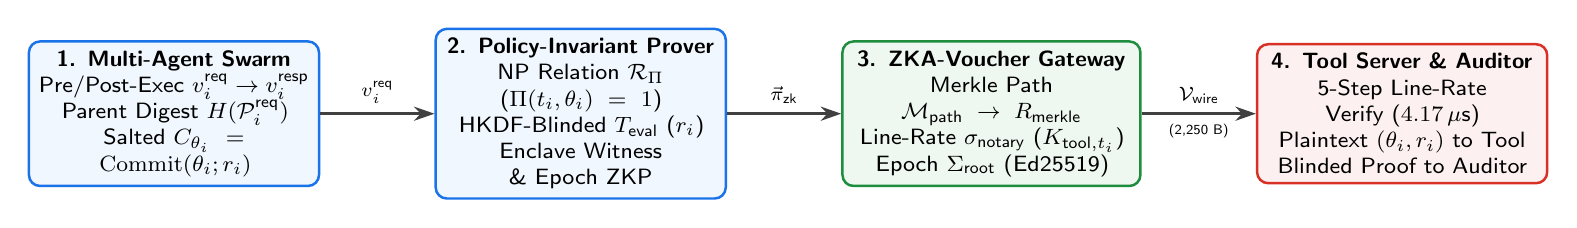
\begin{tikzpicture}[
    node distance=0.9cm and 1.45cm,
    box/.style={rectangle, rounded corners=4pt, draw=googleblue, line width=0.9pt, fill=googleblue!6, text width=3.45cm, align=center, minimum height=1.55cm, font=\footnotesize\sffamily},
    greenbox/.style={rectangle, rounded corners=4pt, draw=googlegreen, line width=0.9pt, fill=googlegreen!7, text width=3.55cm, align=center, minimum height=1.55cm, font=\footnotesize\sffamily},
    redbox/.style={rectangle, rounded corners=4pt, draw=googlered, line width=0.9pt, fill=googlered!7, text width=3.45cm, align=center, minimum height=1.55cm, font=\footnotesize\sffamily},
    arrow/.style={-{Stealth[length=2.6mm, width=1.8mm]}, line width=0.9pt, draw=black!75}
]
\node[box] (n1) {\textbf{1. Multi-Agent Swarm}\\Pre/Post-Exec $v_i^{\text{req}} \to v_i^{\text{resp}}$\\Parent Digest $H(\mathcal{P}_i^{\text{req}})$\\Salted $C_{\theta_i} = \operatorname{Commit}(\theta_i; r_i)$};
\node[box, right=of n1] (n2) {\textbf{2. Policy-Invariant Prover}\\NP Relation $\mathcal{R}_{\Pi}$ ($\Pi(t_i, \theta_i)=1$)\\HKDF-Blinded $T_{\text{eval}}$ ($r_i$)\\Enclave Witness \& Epoch ZKP};
\node[greenbox, right=of n2] (n3) {\textbf{3. ZKA-Voucher Gateway}\\Merkle Path $\mathcal{M}_{\text{path}} \to R_{\text{merkle}}$\\Line-Rate $\sigma_{\text{notary}}$ ($K_{\text{tool}, t_i}$)\\Epoch $\Sigma_{\text{root}}$ (Ed25519)};
\node[redbox, right=of n3] (n4) {\textbf{4. Tool Server \& Auditor}\\5-Step Line-Rate Verify ($4.17\,\mu\text{s}$)\\Plaintext $(\theta_i, r_i)$ to Tool\\Blinded Proof to Auditor};

\draw[arrow] (n1) -- node[above, font=\scriptsize\sffamily] {$v_i^{\text{req}}$} (n2);
\draw[arrow] (n2) -- node[above, font=\scriptsize\sffamily] {$\vec{\pi}_{\text{zk}}$} (n3);
\draw[arrow] (n3) -- node[above, font=\scriptsize\sffamily] {$\mathcal{V}_{\text{wire}}$} node[below, font=\tiny\sffamily] {(2,250 B)} (n4);
\end{tikzpicture}%
}
\caption{End-to-End Architecture of the Agent-Notary Cryptographic Non-Repudiation Pipeline. Multi-agent tool invocations mint $v_i^{\text{req}}$ pre-execution (and append $v_i^{\text{resp}}$ upon tool return) with randomized blinding commitments ($C_{\theta_i}$), are certified via Dual-Tier Blinded Policy-Invariant Attestations ($\vec{\pi}_{\text{zk}}$), encapsulated in wire-level ZKA-Vouchers, and verified in $4.17\,\mu\text{s}$ at line rate alongside Ed25519 and Pedersen/Bulletproof frontier epoch anchoring.}
\label{fig:notary_arch}
\end{figure*}

\subsection{The Zero-Knowledge Action Attestation Voucher (ZKA-Voucher)}
As illustrated in Figure~\ref{fig:notary_arch}, when an agent invokes an external tool, the Agent-Notary Gateway intercepts the invocation frame, verifies $\Pi(t_i, \theta_i) = 1$, and synthesizes a canonical \textbf{ZKA-Voucher}:
\begin{equation}
\begin{split}
\mathcal{V}_{\text{wire}} = \langle &\text{vid}, R_{\text{merkle}}, H_{\text{leaf}}, H(\mathcal{P}_i^{\text{req}}), C_{\theta_i}, r_i^{\text{intra}}, a_i, t_i, \lambda_i, \\
&\tau_{\text{ns}}, \vec{\pi}_{\text{zk}}, \mathcal{M}_{\text{path}}, \sigma_{\text{notary}}, \text{kid}_{\text{notary}}, \text{pk}_{\text{notary}} \rangle
\end{split}
\end{equation}
where $\text{vid} \equiv \text{id}_i^{\text{req}}$ is the unique vertex/voucher UUID, $R_{\text{merkle}} \equiv R_T$ is the active session-sharded frontier root at dispatch snapshot $T$, $H_{\text{leaf}} \equiv H(v_i^{\text{req}})$, $H(\mathcal{P}_i^{\text{req}})$ is the 32-byte parent-set digest required by the verifier to reconstruct candidate digest $H_{\text{leaf}}^*$ (throughout, superscript $(\cdot)^*$ denotes a candidate value recomputed independently by the verifier), $r_i^{\text{intra}} \equiv r_i$ is the 32-byte blinding opening carried exclusively on the intra-cluster hop to the tool server and stripped before persisting $\mathcal{V}_{\text{wire}}$ to external audit stores, $\tau_{\text{ns}}$ is the synchronized monotonic wall-clock timestamp, $\vec{\pi}_{\text{zk}} \triangleq \langle \pi_i, T_{\text{eval}}, C_{\text{circuit}}, x_i, \mathrm{id}_{\Pi}, \texttt{session\_id}, \texttt{escrow\_mode} \rangle$ is the immutable hot-path policy-attestation bundle (with $\mathrm{id}_{\Pi}$ in normal roman weight, and a 1-byte $\operatorname{encode}_8(\texttt{escrow\_mode}) \in \{\mathtt{0x00},\mathtt{0x01}\}$ flag signaling whether the destination verifier must hold irreversible mutations in provisional escrow until Spanner epoch anchoring completes; at $100\,\text{ms}$ epoch anchoring, Ristretto255 Pedersen commitments $\vec{C}_{\text{ped}}$ and Bulletproof transcript $\pi_i^{\text{pub}}$ are attached as companion archival fields in the epoch log without mutating $\operatorname{encode}(\vec{\pi}_{\text{zk}})$), $\mathcal{M}_{\text{path}}$ is the binary Merkle inclusion path, and $\sigma_{\text{notary}}$ is the cryptographic gateway authenticator.

\textbf{Dual-Mode Cryptographic Trust Model \& Per-Tool Key Isolation:} To reconcile sub-$5\,\mu\text{s}$ verification with third-party non-repudiation while preventing lateral voucher forgery across intra-cluster microservices:
\begin{enumerate}
    \item \textbf{Service-Bound Intra-Cluster Line-Rate Attestation:} Rather than sharing a single master secret $K_{\text{gateway}}$ across tool servers, the gateway enclave derives a service-specific verification key for each destination tool $t_i$ via RFC 5869 HKDF-SHA256 (where two-argument notation $\operatorname{HKDF-SHA256}(\text{ikm}, \allowbreak \text{info})$ denotes $\operatorname{HKDF-Expand}(\allowbreak\operatorname{HKDF-Extract}(\text{salt}_{\text{notary}}, \allowbreak \text{ikm}), \allowbreak \text{info}, \ell_{\text{out}} = 32)$ with $32$-octet output length and fixed domain-separated salt $\text{salt}_{\text{notary}}$):
    \begin{equation}
    \begin{split}
    K_{\text{tool}, t_i} = \operatorname{HKDF-SHA256}\big(&K_{\text{gateway}}, \\
    &\operatorname{lp}(t_i) \parallel \operatorname{lp}(\text{kid}_{\text{notary}})\big)
    \end{split}
    \end{equation}
    Each intra-cluster tool server $t_i$ is provisioned strictly with its scoped 32-byte key $K_{\text{tool}, t_i}$, ensuring that a compromised tool server $t_A$ cannot forge authenticators or witnesses for any other tool $t_B \neq t_A$ (while $\text{kid}_{\text{notary}}$ resolves to $\text{pk}_{\text{notary}}$ in the $\mathcal{Q}_{\text{TEE}}$-attested gateway key registry and $\text{pk}_{\text{notary}}$ is carried inline for cross-checked external verification). Using length-prefixed serialization $\operatorname{lp}(s) = \operatorname{encode}_{64}(|s|) \parallel s$ for variable-length strings and explicit 1-byte domain tags $\mathtt{0x0D}$ and $\mathtt{0x0E}$ for the bundle digests $\operatorname{SHA256}(\mathtt{0x0D} \parallel \operatorname{encode}(\vec{\pi}_{\text{zk}}))$---where $\operatorname{encode}(\vec{\pi}_{\text{zk}}) \triangleq \pi_i \parallel T_{\text{eval}} \parallel C_{\text{circuit}} \parallel x_i \parallel \operatorname{lp}(\mathrm{id}_{\Pi}) \parallel \operatorname{lp}(\texttt{session\_id}) \parallel \operatorname{encode}_8(\texttt{escrow\_mode})$---and $\operatorname{SHA256}(\mathtt{0x0E} \parallel \operatorname{encode}(\mathcal{M}_{\text{path}}))$---where $\operatorname{encode}(\mathcal{M}_{\text{path}}) \triangleq \operatorname{encode}_{64}(|\mathcal{V}_{\text{frontier}}|) \parallel \operatorname{encode}_8(d_{\text{active}}) \parallel \operatorname{encode}_{32}(\texttt{dir\_mask}) \parallel S_1 \parallel \dots \parallel S_{d_{\text{active}}}$ over the $d_{\text{active}}$ active 32-byte sibling digests---$\sigma_{\text{notary}}$ authenticates all persistent voucher fields while intentionally excluding $r_i^{\text{intra}}$ so that stripping $r_i^{\text{intra}}$ prior to external archival preserves $\sigma_{\text{notary}}$ (while intra-cluster verifiers authenticate $r_i^{\text{intra}}$ via $C_{\theta_i}^* = C_{\theta_i}$ in Step~3, and external auditors treat $\pi_i$ and $C_{\theta_i}$ as opaque 32-byte inputs when recomputing Eq.~6):
    \begin{equation}
    \begin{split}
    \sigma_{\text{notary}} &= \operatorname{HMAC-SHA256}_{K_{\text{tool}, t_i}}\Big(\operatorname{lp}(\text{vid}) \parallel R_{\text{merkle}} \\
    &\parallel H_{\text{leaf}} \parallel H(\mathcal{P}_i^{\text{req}}) \parallel C_{\theta_i} \parallel \operatorname{lp}(a_i) \parallel \operatorname{lp}(t_i) \\
    &\parallel \operatorname{encode}_{64}(\lambda_i) \parallel \operatorname{encode}_{64}(\tau_{\text{ns}}) \\
    &\parallel \operatorname{SHA256}(\mathtt{0x0D} \parallel \operatorname{encode}(\vec{\pi}_{\text{zk}})) \\
    &\parallel \operatorname{SHA256}(\mathtt{0x0E} \parallel \operatorname{encode}(\mathcal{M}_{\text{path}})) \\
    &\parallel \operatorname{lp}(\text{kid}_{\text{notary}}) \parallel \text{pk}_{\text{notary}}\Big)
    \end{split}
    \end{equation}
    \item \textbf{Third-Party Public Non-Repudiation \& Cross-Domain Dispatch:} For external auditors (who never possess $K_{\text{gateway}}$ or $K_{\text{tool}, t_i}$), the gateway signs frontier epoch roots and policy attestation transcripts every $\Delta_{\text{epoch}} = 100\,\text{ms}$ using an asymmetric Ed25519 private key~\cite{bernstein2012ed25519} protected inside the Confidential VM enclave and bound to the enclave binary measurement via an AMD SEV-SNP hardware remote attestation quote $\mathcal{Q}_{\text{TEE}}$. Using 1-byte domain prefix $\mathtt{0x08}$, the batch epoch signature is $\Sigma_{\text{root}} = \operatorname{Sign}_{\text{Ed25519}}\big(\text{sk}_{\text{notary}}, \mathtt{0x08} \parallel \operatorname{encode}_{64}(\text{seq}_{\text{epoch}}) \parallel R_{\text{merkle}} \parallel \operatorname{encode}_{64}(\tau_{\text{epoch}}) \parallel H_{\text{epoch}}(\vec{\pi}_{\text{zk}})\big)$, where $H_{\text{epoch}}(\vec{\pi}_{\text{zk}})$ is the $\mathtt{0x05}$ cardinality-enveloped RFC 6962 Merkle root over the epoch's chronologically ordered per-call commitment-equivalence leaves $L_{\text{eq}, i}^{\text{epoch}} = \operatorname{SHA256}\big(\mathtt{0x0C} \parallel H_{\text{leaf}} \parallel \operatorname{encode}_8(\texttt{escrow\_mode}) \parallel C_{\text{circuit}} \parallel x_i \parallel C_{\theta_i} \parallel D_{\text{ped}, i} \parallel T_{\text{eval}} \parallel D_{\text{pub}, i}\big)$ with sub-tagged proof digests $D_{\text{ped}, i} \triangleq \operatorname{SHA256}(\mathtt{0x0F} \parallel \mathtt{0x01} \parallel \operatorname{encode}_{64}(m) \parallel \vec{C}_{\text{ped}})$ (where $\vec{C}_{\text{ped}} = C_{\text{ped}, 1} \parallel \dots \parallel C_{\text{ped}, m}$ is the deterministic concatenation of the $m$ 32-byte canonical Ristretto255 commitment encodings) and $D_{\text{pub}, i} \triangleq \operatorname{SHA256}(\mathtt{0x0F} \parallel \mathtt{0x02} \parallel \pi_i^{\text{pub}})$, verifiable publicly alongside $\mathcal{Q}_{\text{TEE}}$ using $\text{pk}_{\text{notary}}$. Under domain prefix $\mathtt{0x09}$ (partitioned into sub-tags $\mathtt{0x09} \parallel \mathtt{0x00}$ for gateway cross-domain dispatch, $\mathtt{0x09} \parallel \mathtt{0x01}$ for verifier-signed execution/error receipts, and $\mathtt{0x09} \parallel \mathtt{0x02}$ for verifier-signed \texttt{NOT\_SEEN} inquiry receipts under the destination verifier's $\mathcal{Q}_{\text{TEE}}$-attested Ed25519 key $\text{sk}_{\text{verifier}, t_i}$), when a tool call crosses an organizational boundary synchronously to an external tool server lacking $K_{\text{tool}, t_i}$ (which still receives $(\theta_i, r_i^{\text{intra}})$ in plaintext to execute $t_i(\theta_i)$ and run Step~3), the gateway attaches an immediate on-demand Ed25519 signature $\Sigma_{\text{cross}} = \operatorname{Sign}_{\text{Ed25519}}\big(\text{sk}_{\text{notary}}, \mathtt{0x09} \parallel \mathtt{0x00} \parallel R_{\text{merkle}} \parallel H_{\text{leaf}} \parallel \operatorname{encode}_{64}(\tau_{\text{ns}}) \parallel \operatorname{encode}_8(\texttt{escrow\_mode}) \parallel L_{\text{eq}, i}^{\text{sync}}\big)$ via \texttt{x-agent-notary-crossdomain-sig} (verifiable in $62.4\,\mu\text{s}$ by the destination tool server; on the default $62.4\,\mu\text{s}$ cross-domain path where synchronous ZKP attachment is omitted, $\Sigma_{\text{cross}}$ under prefix $\mathtt{0x09} \parallel \mathtt{0x00}$ serves as the enclave's direct attestation of $\Pi(t_i, \theta_i) = 1$ with $L_{\text{eq}, i}^{\text{sync}}$ setting $D_{\text{ped}, i} = D_{\text{pub}, i} = 0^{256}$, while the $100\,\text{ms}$ epoch root $H_{\text{epoch}}(\vec{\pi}_{\text{zk}})$ commits $L_{\text{eq}, i}^{\text{epoch}}$ with populated $(D_{\text{ped}, i}, D_{\text{pub}, i})$ and the signed epoch release bundle provides $(D_{\text{ped}, i}, D_{\text{pub}, i})$ alongside the RFC 6962 inclusion path so an escrow-holding verifier can reconstruct $L_{\text{eq}, i}^{\text{epoch}}$ from its cached $(H_{\text{leaf}}, \texttt{escrow\_mode}, C_{\text{circuit}}, x_i, C_{\theta_i}, T_{\text{eval}})$; when synchronous cross-domain ZKP attachment is enabled, $L_{\text{eq}, i}^{\text{sync}} = L_{\text{eq}, i}^{\text{epoch}}$, and full third-party zero-knowledge verification of $\Sigma_{\text{root}} + \pi_i^{\text{pub}}$ when $(\theta_i, r_i^{\text{intra}})$ is withheld requires $840\,\mu\text{s}$).
\end{enumerate}

\textbf{Dual-Tier Blinded Policy-Invariant Attestation Engine:} To certify that private parameters satisfy policy constraints ($\Pi(t_i, \theta_i) = 1$) without exposing raw parameter values or allowing offline dictionary brute-forcing by external auditors, the engine formalizes the NP statement-witness relation over attribute scalars $v_{i,k} \in \mathbb{Z}_q$ indexed in deterministic RFC 8785 JCS lexicographical JSON pointer order $k \in \{1, \dots, m\}$ (where numeric attributes are mapped to integer base units $0 \le L_{\min} \le v_{i,k} = \lfloor \theta_{i,k} \cdot 10^{s_k} \rceil \le L_{\max} < 2^{64}$ via per-attribute fixed-point decimal scaling exponents $s_k \in \mathbb{N}$ committed inside $C_{\text{circuit}}$, and $v_{i,k} = u_{i,k} \triangleq \operatorname{SHA256}(\theta_{i,k}) \bmod q$ for public string/URI attributes, or $u_{i,k} \triangleq \operatorname{HKDF-Expand}_{512}\big(\operatorname{HMAC-SHA256}(k_{\text{audit}}, \mathtt{0x10} \parallel \operatorname{lp}(\mathrm{id}_{\Pi}) \parallel \operatorname{encode}_{32}(k) \parallel \operatorname{lp}(\theta_{i,k})), \text{``allowlist-scalar''}\big) \bmod q$ when allowlist literals are confidential, interpreting 32-byte/64-byte hash outputs as unsigned little-endian integers before reduction modulo $q$):
\begin{equation}
\begin{split}
\mathcal{R}_{\Pi} = \Big\{ &\big\langle(t_i, C_{\theta_i}, \vec{C}_{\text{ped}}, x_i), (\theta_i, r_i)\big\rangle \;\Big|\; C_{\theta_i} = \operatorname{Commit}(\theta_i; r_i) \\
&\land\; \Big(\bigwedge_{k=1}^{m} C_{\text{ped}, k} = g^{v_{i,k}} h^{r_{i,k}}\Big) \land \Pi(t_i, \theta_i) = 1 \Big\}
\end{split}
\end{equation}
where $x_i = \operatorname{SHA256}(\mathtt{0x0A} \parallel \operatorname{lp}(a_i) \parallel \operatorname{lp}(t_i) \parallel \operatorname{lp}(\texttt{session\_id}))$ is the domain-separated public context and $C_{\text{circuit}} = \operatorname{SHA256}(\mathtt{0x0B} \parallel \operatorname{lp}(\mathrm{id}_{\Pi}) \parallel \operatorname{lp}(\text{type}_{\Pi}) \parallel \operatorname{lp}(\text{expr}_{\Pi}))$ is the policy circuit descriptor exported alongside $(\mathrm{id}_{\Pi}, \text{type}_{\Pi}, \text{expr}_{\Pi})$ in the public audit transcript (where the canonical circuit expression string $\text{expr}_{\Pi}$ serializes and commits to per-attribute scaling exponents $s_k$, $\text{kid}_{\text{audit}}$, and the expanded monic polynomial coefficients $c_0, \dots, c_{d-1}$ of $P(u) = \prod_{w \in \mathcal{U}_{\text{allow}}}(u - w) = u^d + \sum_{j=0}^{d-1} c_j u^j$ when $\mathcal{U}_{\text{allow}}$ is confidential, where $k_{\text{audit}}$ is provisioned via KMS gated by $\mathcal{Q}_{\text{TEE}}$). Because low-degree polynomials over $\mathbb{Z}_q$ can be factored algebraically via Cantor-Zassenhaus in $O(d^2 \log q)$ field operations to recover their roots $w \in \mathcal{U}_{\text{allow}}$, confidential allowlist string secrecy rests strictly on the PRF security of $\mathtt{0x10}$-tagged $\operatorname{HMAC-SHA256}(k_{\text{audit}}, \cdot)$, which maps each allowlist literal to a pseudorandom root $w \in \mathbb{Z}_q$ irreversible without $k_{\text{audit}}$. Furthermore, to prevent dictionary brute-forcing on low-entropy parameters $\theta_i$ (such as categorical enums or small numeric scalars), the blinded evaluation token $T_{\text{eval}}$ is keyed using an HKDF-derived blinding key extracted directly from the secret 256-bit commitment randomness $r_i \xleftarrow{\$} \{0,1\}^{256}$ rather than public identifiers:
\begin{equation}
\begin{split}
k_{\text{blind}, i} &= \operatorname{HKDF-SHA256}\big(r_i, \;\operatorname{lp}(\mathrm{id}_{\Pi}) \parallel \operatorname{lp}(\text{vid})\big), \\
T_{\text{eval}} &= \operatorname{HMAC-SHA256}\big(k_{\text{blind}, i}, \;\operatorname{CanonicalJSON}(\theta_i)\big)
\end{split}
\end{equation}
Because $r_i$ has 256 bits of min-entropy and is withheld from external auditors, $(C_{\theta_i}, T_{\text{eval}}, \vec{C}_{\text{ped}})$ is computationally hiding under the PRF security of HKDF/HMAC-SHA256 (and binds $T_{\text{eval}}$ inside $L_{\text{eq}, i}$ for intra-cluster/epoch audit cross-checking). Attestation operates across two complementary tiers:
\begin{itemize}
    \item \emph{Tier 1 (Hot-Path Enclave Policy Witness, $0.77\,\mu\text{s}$):} On the synchronous tool-call critical path, no elliptic-curve scalar multiplications are executed. The trusted gateway enclave evaluates $\Pi(t_i, \theta_i) = 1$ in memory and issues a service-bound witness token $\pi_i = \operatorname{HMAC-SHA256}_{K_{\text{tool}, t_i}}(C_{\text{circuit}} \parallel x_i \parallel C_{\theta_i} \parallel T_{\text{eval}} \parallel \mathtt{0x01})$ (where trailing byte $\mathtt{0x01}$ encodes the compliance bit $\Pi(t_i, \theta_i) = 1$). Intra-cluster tool servers receive $(\theta_i, r_i^{\text{intra}})$ in plaintext to execute the operation, recomputing $C_{\theta_i}^*$, $H_{\text{leaf}}^*$ ($0.72\,\mu\text{s}$) and $k_{\text{blind}, i}^*$, $T_{\text{eval}}^*$, $\pi_i^*$ ($0.77\,\mu\text{s}$) without any elliptic-curve overhead.
    \item \emph{Tier 2 (Hybrid TEE-Bound Commitment Equivalence \& Zero-Knowledge Epoch Proofs):} To provide public auditability to untrusted third-party auditors when $(\theta_i, r_i^{\text{intra}})$ and $K_{\text{tool}, t_i}$ are withheld, the gateway asynchronously compiles an algebraic zero-knowledge proof $\pi_i^{\text{pub}}$ over the prime-order Ristretto255 group ($\mathbb{G}$ of order $q = 2^{252} + 27742317777372353535851937790883648493$) during $100\,\text{ms}$ epoch anchoring. For each of the $m$ policy-constrained JSON AST attributes ($v_{i,k} = \lfloor \theta_{i,k} \cdot 10^{s_k} \rceil \in \mathbb{Z}_q$ for numeric fields and $v_{i,k} = u_{i,k}$ for string/URI fields), the gateway expands a 64-byte (512-bit) HKDF output before little-endian reduction modulo $q$, $r_{i,k} = \operatorname{HKDF-Expand}_{512}(r_i, \text{``pedersen''} \parallel \operatorname{encode}_{64}(k)) \bmod q$ (eliminating modulo bias to $< 2^{-256}$), and forms Pedersen commitments $C_{\text{ped}, k} = g^{v_{i,k}} h^{r_{i,k}} \in \mathbb{G}$~\cite{pedersen1991non}. Numeric bounds $v_{i,k} \in [L_{\min}, L_{\max}] \subseteq [0, 2^{64})$ are proven via dual 64-bit Bulletproof bit-decomposition constraints~\cite{bunz2018bulletproofs} on lower-slack commitment $C_{\text{ped}, k} g^{-L_{\min}} = g^{v_{i,k} - L_{\min}} h^{r_{i,k}}$ and upper-slack commitment $g^{L_{\max}} C_{\text{ped}, k}^{-1} = g^{L_{\max} - v_{i,k}} h^{-r_{i,k}}$ ($128$ multiplication gates, where each $C_{\text{ped},k}$ is bound as a single R1CS variable commitment from which the verifier homomorphically derives both slack points inside the linear constraint system during multi-scalar multiplication), while finite allowlist set-membership polynomials $P(u_{i,k}) = 0 \pmod q$ are evaluated via Horner's rule ($z_1 = c_{d-1} + u_{i,k}$ as a free linear addition since monic $c_d = 1$, and $z_j = c_{d-j} + u_{i,k} z_{j-1}$ for $j=2,\dots,d$ constrained to $z_d = 0$, requiring $d - 1 = |\mathcal{U}_{\text{allow}}| - 1$ multiplication gates) within a single unified Bulletproofs R1CS instance padded to $N_{\text{bp}} = 256$ gates over independent generators $\vec{g}, \vec{h} \in \mathbb{G}^{256}$ derived via SHAKE256 hash-to-curve (\text{``Agent-Notary-BP-v1''}) with $(x_i, C_{\text{circuit}}, \text{vid})$ bound into the Fiat-Shamir challenge hash~\cite{fiat1986how} (yielding $2\log_2(256) + 8 = 24$ Ristretto255 elements: $768$~B full 24-element transcript hashed under $\mathtt{0x0F}\parallel\mathtt{0x02}$ in $D_{\text{pub},i}$, or $704$~B in compact wire layout omitting the two second-phase wire commitment points $(A_{I2}, A_{O2}) = (\mathcal{O}_{\mathbb{G}}, \mathcal{O}_{\mathbb{G}})$ unused by single-phase circuits). We explicitly frame Tier~2 as a \emph{hybrid TEE-cryptographic trust model}: for external third-party auditors lacking $(\theta_i, r_i^{\text{intra}})$, $\mathcal{Q}_{\text{TEE}}$ shrinks the trusted enclave surface from the dynamic policy evaluator $\Pi$ to the static JSON-to-Pedersen extraction stub that binds $C_{\theta_i}$ to $\vec{C}_{\text{ped}}$ inside $L_{\text{eq}, i}^{\text{epoch}}$ (where, to eliminate JSON parser differentials between the gateway and destination tool servers, the stub first canonicalizes the incoming request into a single RFC 8785 JCS byte buffer---rejecting duplicate keys, non-shortest UTF-8 sequences, IEEE-754 \texttt{NaN}/\texttt{Infinity} tokens, and trailing bytes---computes $C_{\theta_i}$ over that exact JCS buffer, extracts $v_{i,k}$ directly from the single parsed JCS AST without re-parsing, and transmits those exact JCS-canonicalized bytes $\operatorname{CanonicalJSON}(\theta_i)$ over the wire), whereas intra-cluster tool servers and authorized dispute-resolution auditors holding $(\theta_i, r_i^{\text{intra}})$ recompute $\vec{C}_{\text{ped}}^*$ directly via $(v_{i,k}, r_{i,k})$ without trusting $\mathcal{Q}_{\text{TEE}}$ (from $(\theta_i, r_i^{\text{intra}})$ alone for numeric attributes and public allowlists, or alongside KMS-provisioned $k_{\text{audit}}$ when confidential allowlists are active; external cross-domain tool servers that do not share the caller's confidential $k_{\text{audit}}$ recompute $C_{\text{ped}, k}^*$ directly for numeric and public-allowlist attributes while hashing wire-supplied confidential-allowlist commitments inside $\vec{C}_{\text{ped}}$ under $\mathcal{Q}_{\text{TEE}}$-attested $\Sigma_{\text{cross}}$; furthermore, to mitigate single-vendor TEE microarchitectural or side-channel risk when $(\theta_i, r_i^{\text{intra}})$ are permanently withheld from external public auditors, the $\sim 400$-LoC memory-safe Rust JCS extraction stub supports optional $2$-of-$3$ heterogeneous multi-vendor TEE quorum co-signing---spanning AMD SEV-SNP, Intel TDX, and AWS Nitro Enclaves via threshold Ed25519 FROST signatures~\cite{komlo2020frost} over $L_{\text{eq}, i}^{\text{epoch}}$---or asynchronous off-path lookup-argument SNARK equivalence proofs~\cite{setty2024jolt} [e.g., Plonky3/Lasso-Jolt byte-table lookups proving JCS parsing and SHA-256 $C_{\theta_i} \leftrightarrow \vec{C}_{\text{ped}}$ equivalence in $\approx 180$--$320\,\text{ms}$ on GPU/FPGA audit workers] without altering the $4.17\,\mu\text{s}$ hot-path voucher format).
\end{itemize}

\subsection{Wire Protocol Encapsulation}
The ZKA-Voucher is serialized into a compact Base64 JSON token and injected into transport metadata:
\begin{itemize}
    \item \textbf{gRPC Metadata}: Attached as header \texttt{x-agent-notary-voucher}.
    \item \textbf{MCP JSON-RPC Frames}: Embedded into the top-level \texttt{headers} dictionary of \texttt{tools/call} requests, adhering to RFC 9421 header conventions~\cite{backman2024rfc9421}.
\end{itemize}
To ensure a predictable header footprint across active per-session frontier depths $\lceil \log_2 |\mathcal{V}_{\text{frontier}}| \rceil \in \{3, 4, 5\}$, the wire serializer normalizes $\mathcal{M}_{\text{path}}$ to a canonical 4-slot sibling array (padding depth-3 paths with a zeroed 64-byte hex slot; unpadded paths across depths $\{3, 4, 5\}$ span $1{,}624$--$1{,}752$~B raw JSON, and if an active session burst ever exceeds 4 sibling slots [$d_{\text{active}} > 4$, e.g., $d_{\text{active}} = 5$ at $17 \le |\mathcal{V}_{\text{frontier}}| \le 32$], the gateway either triggers an inline mini-epoch compaction of completed sub-branches or spills sibling hashes $S_5, \dots, S_{d_{\text{active}}}$ into an optional companion header \texttt{x-agent-notary-path-ext} at $+64$~B hex / $+32$~B raw per level above $4$, authenticated inside $\operatorname{encode}(\mathcal{M}_{\text{path}})$ under $\mathtt{0x0E}$). Across the $1{,}000$ benchmark traces under canonical 4-slot framing, raw JSON vouchers average $1{,}687.5$~B (ranging from $1{,}686$~B to $1{,}695$~B across variable-length tool names $t_i$). For a representative voucher ($1{,}688$~B raw JSON), the payload decomposes into $1{,}476$~B of field bundles (including nested sub-object delimiters)---metadata ($\text{vid}, a_i, t_i, \lambda_i, \tau_{\text{ns}}, \text{kid}_{\text{notary}}, \text{pk}_{\text{notary}}$) $= 280$~B, vertex/root hex digests ($R_{\text{merkle}}, H_{\text{leaf}}, C_{\theta_i}$) $= 192$~B, parent digest and intra-cluster salt ($H(\mathcal{P}_i^{\text{req}}), r_i^{\text{intra}}$: two $64$~B hex digests plus $2$~B delimiter) $= 130$~B, 4-slot Merkle path ($\mathcal{M}_{\text{path}}$: four $64$~B sibling hex digests plus $34$~B encoding the left/right bitmask, active depth, and frontier cardinality $|\mathcal{V}_{\text{frontier}}|$ for Eq.~7) $= 290$~B, hot-path policy attestation bundle ($\vec{\pi}_{\text{zk}}$) $= 520$~B, and authenticator ($\sigma_{\text{notary}}$: $64$~B hex decoded to $32$ raw bytes prior to HMAC verification) $= 64$~B---plus $212$~B of top-level JSON keys and delimiters. Base64 encoding yields $\lceil 1{,}688 \times 4 / 3 \rceil = 2{,}251$~B unpadded ($4\lceil 1{,}688 / 3 \rceil = 2{,}252$~B padded), with an empirical mean wire footprint of $2{,}250$~bytes (P50: $2{,}248$~B, P95: $2{,}256$~B, P99: $2{,}260$~B). Stripping $r_i^{\text{intra}}$ ($66$~B with delimiter) yields $1{,}622$~B raw JSON for external archival; when synchronous cross-domain ZKP attachment is enabled ($m=2$), \texttt{x-agent-notary-crossdomain-sig} adds $832$~B raw binary ($64$~B $\Sigma_{\text{cross}}$, $64$~B $\vec{C}_{\text{ped}}$, and $704$~B compact $\pi_i^{\text{pub}}$; $1{,}112$~B padded Base64).

\subsection{Line-Rate Intra-Cluster Verification Pipeline}
{\emergencystretch=6em
When a destination tool server receives an invocation, the embedded verifier executes five invariant checks in strictly bounded time ($< 50\,\mu\text{s}$ on the intra-cluster symmetric hot path):
\begin{enumerate}
    \item \textbf{Key Trust and Authenticator Invariant}: Validates $(\text{kid}_{\text{notary}},\allowbreak \text{pk}_{\text{notary}})$ against the local or $\mathcal{Q}_{\text{TEE}}$-attested gateway key registry and evaluates $\sigma_{\text{notary}}$ using service-scoped $K_{\text{tool}, t_i}$ (or on the synchronous cross-domain path, first executes the read-only $0.12\,\mu\text{s}$ Step~2 freshness/replay check, $0.72\,\mu\text{s}$ Step~3 commitment check $C_{\theta_i}^* = C_{\theta_i}$ and $H_{\text{leaf}}^* = H_{\text{leaf}}$, and Step~5 $x_i^*,\allowbreak k_{\text{blind}, i}^*,\allowbreak T_{\text{eval}}^*$ derivation and $L_{\text{eq}, i}^{\text{sync}*}$ reconstruction to fast-reject stale or malformed frames and return cached retry receipts before completing the $62.4\,\mu\text{s}$ Ed25519 $\Sigma_{\text{cross}}$ verification over $L_{\text{eq}, i}^{\text{sync}*}$ under registry-validated $\text{pk}_{\text{notary}}$).
    \item \sloppy\textbf{Timestamp Freshness and Anti-Replay}: Asserts $|\tau_{\text{now}} - \tau_{\text{ns}}| \le \Delta_{\text{TTL}}$ ($5\text{ minutes}$) and queries $\text{vid}$ against an in-memory lock-free replay cache pairing a 4-way set-associative Robin Hood hash table indexed by $\text{vid}$ ($0.12\,\mu\text{s}$ $O(1)$ lookup included within the $0.68\,\mu\text{s}$ Steps~1--2 check) with a circular FIFO timestamp eviction ring sized to satisfy $N_{\text{ring}} > \lambda_{\text{peak}} \cdot \Delta_{\text{TTL}}$ (default $N_{\text{ring}} = 2^{20}$ slots covering $\lambda_{\text{peak}} \le 3{,}495\text{ req/s}$ over $\Delta_{\text{TTL}} = 300\text{ s}$ in $32\text{ MB}$, scaling to $N_{\text{ring}} \in [2^{26},\allowbreak 2^{27}]$ or sharded per-core rings for $> 200\text{k req/s}$ line-rate replicas and failing closed if the oldest ring slot is younger than $\Delta_{\text{TTL}}$). To prevent in-transit tampering of unauthenticated plaintext $(\theta_i,\allowbreak r_i^{\text{intra}})$ from poisoning $\text{vid}$ before Step~3, state-mutating $\text{vid}$ insertion is deferred until Steps~3--5 (and $\Sigma_{\text{cross}}$ on cross-domain calls) succeed and committed via an atomic compare-and-swap (\texttt{insert\_\allowbreak if\_\allowbreak absent}) setting the slot state to \texttt{IN\_\allowbreak FLIGHT} under a bounded execution lease ($\Delta_{\text{exec\_lease}} = 30\text{ s}$) prior to executing $t_i$, transitioning to \texttt{COM\allowbreak PLETED} once the $\text{sk}_{\text{verifier}, t_i}$-signed ($\mathtt{0x09} \parallel \mathtt{0x01}$) execution receipt is appended (or transitioning via an exception guard to \texttt{ABORTED\_\allowbreak EVICTED} with a signed failure receipt if local execution of $t_i$ faults or times out, preventing stuck \texttt{IN\_\allowbreak FLIGHT} slots): if a retry carrying $(H_{\text{leaf}},\allowbreak \text{vid})$ hits an active \texttt{IN\_\allowbreak FLIGHT} slot it awaits completion, and if it hits a \texttt{COM\allowbreak PLETED} slot the verifier returns the cached execution receipt idempotently.
    \item \textbf{Parameter \& Leaf Binding Invariant}: Asserts $t_i$ matches the local tool identity and reconstructs $C_{\theta_i}^*$ and $H_{\text{leaf}}^*$ via Eqs.~(2) and (6) from incoming $\theta_i, r_i^{\text{intra}}$ and voucher fields $(\text{vid},\allowbreak a_i,\allowbreak \lambda_i,\allowbreak H(\mathcal{P}_i^{\text{req}}),\allowbreak t_i,\allowbreak H_{\text{pending}},\allowbreak \pi_i)$ (where cross-domain verifiers treat $\pi_i$ as an opaque 32-byte field), asserting $C_{\theta_i}^* = C_{\theta_i}$ and $H_{\text{leaf}}^* = H_{\text{leaf}}$ in $0.72\,\mu\text{s}$.
    \item \textbf{Merkle Frontier Inclusion}: Asserts that all $\max(0, 4 - d_{\text{active}})$ inactive padding slots in the 4-slot JSON $\mathcal{M}_{\text{path}}$ equal $0^{256}$, slices the $d_{\text{active}}$ hex-decoded 32-byte sibling digests $S_1 \parallel \dots \parallel S_{d_{\text{active}}}$ (concatenating any companion \texttt{x-agent-notary-path-ext} slots when $d_{\text{active}} > 4$) when reconstructing the binary $\operatorname{encode}(\mathcal{M}_{\text{path}})$ buffer for Step~1 ($\mathtt{0x0E}$), and evaluates $\mathcal{M}_{\text{path}}$ with $\mathtt{0x00}/\mathtt{0x01}/\mathtt{0x05}$ domain prefixes against $R_{\text{merkle}}$ in $O(\log |\mathcal{V}_{\text{frontier}}|)$ time ($0.58\,\mu\text{s}$), binding $H_{\text{leaf}}$ to the frontier root logged for asynchronous epoch cross-checking.
    \item \textbf{Policy-Invariant Witness \& Escrow Verification}: Asserts $C_{\text{circuit}}$ matches the local administrator-provisioned descriptor for $t_i$ and recomputes $x_i^*, k_{\text{blind}, i}^*, T_{\text{eval}}^*$ from $(r_i^{\text{intra}}, \theta_i, a_i, t_i, \mathrm{id}_{\Pi}, \text{vid}, \texttt{session\_id})$: intra-cluster verifiers assert $\pi_i^* = \pi_i$ in $0.77\,\mu\text{s}$, while cross-domain verifiers reconstruct $L_{\text{eq}, i}^{\text{sync}*}$ (executed prior to Step~1's $\Sigma_{\text{cross}}$ check) and assert $L_{\text{eq}, i}^{\text{sync}*} = L_{\text{eq}, i}^{\text{sync}}$ under $\Sigma_{\text{cross}}$. Specifically, on the default $62.4\,\mu\text{s}$ synchronous cross-domain path, $L_{\text{eq}, i}^{\text{sync}*}$ sets $D_{\text{ped}, i}^* = D_{\text{pub}, i}^* = 0^{256}$; when synchronous cross-domain ZKP attachment is enabled, the cross-domain recipient hashes the wire-supplied $\vec{C}_{\text{ped}}$ and $\pi_i^{\text{pub}}$ into $D_{\text{ped}, i}^*, D_{\text{pub}, i}^*$ inside $L_{\text{eq}, i}^{\text{sync}*}$ (additionally recomputing $C_{\text{ped}, k}^*$ from $(\theta_i, r_i^{\text{intra}})$ for numeric and public-allowlist attributes when plaintext is present, while relying on $\mathcal{Q}_{\text{TEE}}$-attested $\Sigma_{\text{cross}}$ for confidential-allowlist commitments when the caller's $k_{\text{audit}}$ is not shared across organizational boundaries) and verifies the Bulletproof $\pi_i^{\text{pub}}$ ($773.50\,\mu\text{s}$) either when operating as a zero-knowledge boundary gateway from which $(\theta_i, r_i^{\text{intra}})$ is already stripped or to pre-validate the self-contained zero-knowledge proof before stripping $(\theta_i, r_i^{\text{intra}})$ for non-repudiable downstream archival forwarding. If $\texttt{escrow\_mode} = 1$ (authenticated in $\sigma_{\text{notary}} / \Sigma_{\text{cross}}$ or mandated by the local static tool policy table for irreversible mutations), the verifier holds execution until receiving the signed epoch bundle $(\text{seq}_{\text{epoch}}, R_{\text{merkle}}, \tau_{\text{epoch}}, H_{\text{epoch}}(\vec{\pi}_{\text{zk}}), \Sigma_{\text{root}}, D_{\text{ped}, i}, D_{\text{pub}, i})$ and verifying an RFC 6962 Merkle inclusion proof of $L_{\text{eq}, i}^{\text{epoch}}$ in $H_{\text{epoch}}(\vec{\pi}_{\text{zk}})$ under $\Sigma_{\text{root}}$ (failing closed if anchoring exceeds $250\,\text{ms}$, or $350\,\text{ms}$ when extended by an at-most-once $\mathtt{0x12} \parallel \mathtt{0x02}$ Spanner lease-takeover heartbeat).
\end{enumerate}\par}

\section{Empirical Evaluation}
To validate the performance, security, and scalability of Agent-Notary across both transport-layer tampering and multi-agent indirect prompt injections, we executed a two-part empirical evaluation on Google Cloud virtual infrastructure: primary microbenchmarks ran on a \texttt{c3-standard-8} VM instance (Intel Xeon 4th Gen Sapphire Rapids, 3.4~GHz, 8 vCPUs, 32~GB RAM, Debian 12 Linux kernel 6.1), complemented by matched hardware-encrypted Confidential VM validation on a 4th Gen AMD EPYC Genoa \texttt{c3d-standard-8} Confidential VM instance with active AMD SEV-SNP RMP memory encryption and \texttt{/dev/sev-guest} hardware attestation quote generation (where active SEV-SNP memory encryption adds $+1.15\,\mu\text{s}$ to in-memory Tier-1 notarization [$29.60\,\mu\text{s}$] and $+0.18\,\mu\text{s}$ to Tier-1 verification [$4.35\,\mu\text{s}$]; vs.\ $+1.42\,\mu\text{s}$ and $+0.22\,\mu\text{s}$ on a 3rd Gen EPYC Milan \texttt{n2d-standard-8} instance).

\subsection{Part 1: Transport-Layer Tampering \& Replay Cohorts (\texorpdfstring{$N = 1{,}000$}{N = 1,000})}
The first evaluation suite tested $N = 1{,}000$ enterprise traces stratified across five transport and cryptographic cohorts ($n_k$ denoting sub-cohort sizes):
\begin{enumerate}
    \item \textbf{Benign Valid Execution ($n = 193$)}: Legitimate agent actions complying with all financial and infrastructure policies ($\Pi(t_i, \theta_i) = 1$).
    \item \textbf{In-Transit Parameter Escalation ($n = 210$)}: Adversary inflates financial disbursement values or mutates destination cloud storage URIs on the wire after voucher minting ($C_{\theta_i}^* \neq C_{\theta_i}$).
    \item \textbf{Signature Forgery ($n = 198$)}: Attacker alters cryptographic authenticator bytes to simulate a forged gateway voucher.
    \item \textbf{Replay Clock Desynchronization ($n = 199$)}: Attacker replays valid historical vouchers outside the allowable 5-minute TTL window or hits the sliding $\text{vid}$ replay cache.
    \item \textbf{Untrusted Key Forgery ($n = 200$)}: Attacker signs vouchers with an unauthorized or revoked key identifier $\text{kid}_{\text{notary}}$.
\end{enumerate}

\begin{table}[t]
\centering
\caption{Empirical Detection Metrics Across $N = 1{,}000$ Wire Tampering Traces and $N = 300$ Multi-Agent Prompt-Injection Traces}
\label{tab:detection_metrics}
\resizebox{\columnwidth}{!}{%
\begin{tabular}{lccc}
\toprule
\textbf{Evaluation Metric / Benchmark Suite} & \textbf{Measured Value} & \textbf{Clopper-Pearson 95\% CI} & \textbf{Baseline (Unattested)} \\
\midrule
\multicolumn{4}{@{}l}{\textit{\textbf{Panel A: Wire-Level Tampering \& Replay Suite ($N = 1{,}000$ Traces)}}} \\
True Positives (Attacks Blocked, $n=807$) & 807 / 807 & [99.54\%, 100.00\%] & 0 / 807 (0.00\%) \\
True Negatives (Benign Allowed, $n=193$) & 193 / 193 & [98.11\%, 100.00\%] & 193 / 193 (100.00\%) \\[1pt]
Overall Classification Accuracy ($N=1{,}000$)$^{\text{a}}$ & \textbf{100.00\% (1,000/1,000)} & [99.63\%, 100.00\%] & 19.30\% (193/1,000) \\
\midrule
\multicolumn{4}{@{}l}{\textit{\textbf{Panel B: Multi-Agent Prompt-Injection Suite ($N = 300$, AgentDojo/InjecAgent/ASB)}}} \\
Out-of-Policy Injection Block Rate ($\Pi=0, n=200$)$^{\text{b}}$ & \textbf{100.00\% (200/200)} & [98.17\%, 100.00\%] & 31.50\% (63/200) \\
Overall Pre-Execution Block Rate ($N=300$, Static $\Pi=0$)$^{\text{b}}$ & \textbf{66.67\% (200/300)} & [61.02\%, 71.98\%] & 21.00\% (63/300) \\
In-Policy Pre-Execution Block ($\Pi=1, n=100$, Standalone) & \textbf{0.00\% (0/100)} & [0.00\%, 3.62\%] & 0.00\% (0/100) \\
In-Policy Pre-Execution Block ($\Pi=1, n=100$, +Dynamic IFC)$^{\text{b}}$ & \textbf{89.00\% (89/100)} & [81.17\%, 94.38\%] & 0.00\% (0/100) \\
Post-Hoc Attribution: Structural 1-Parent DAG ($|\mathcal{P}_i^{\text{req}}|=1, n=82$) & \textbf{100.00\% (82/82)} & [95.60\%, 100.00\%] & 0.00\% (Mutable Logs) \\
Post-Hoc Attribution: Unconditional Cryptographic Slice (to $\mathcal{P}_i^{\text{req}}$)$^{\text{c}}$ & \textbf{100.00\% (18/18; 20/20 obf.)} & [81.47\%, 100.00\%] / [83.16\%, 100.00\%]$^{\text{c}}$ & 0.00\% (Mutable Logs) \\
Post-Hoc Attribution: Automated 1-of-$k_p$ Exact Pinpointing (AST)$^{\text{c}}$ & \textbf{100.00\% (18/18) / 0.00\% (0/20 obf.)} & [81.47\%, 100.00\%] (18/18)$^{\text{c}}$ & 0.00\% (Mutable Logs) \\
Combined Unconditional Cryptographic Attribution (82/82 + 18/18 $\mathcal{P}_i^{\text{req}}$) & \textbf{100.00\% (100/100)} & [96.38\%, 100.00\%] & 0.00\% (Mutable Logs) \\
Live Benign Swarm Task Utility ($n=193$)$^{\text{b}}$ & \textbf{100.00\% (193/193)} & [98.11\%, 100.00\%] & 100.00\% (193/193) \\
Live Sub-Task Utility Under Attack ($n=200$) & \textbf{98.50\% (197/200)} & [95.68\%, 99.69\%] & 31.50\% (63/200) \\
\bottomrule
\multicolumn{4}{@{}l}{\scriptsize $^{\text{a}}$Unattested baseline accepts all frames ($0/807$ attacks blocked, yielding the $19.30\%$ benign base rate).} \\
\multicolumn{4}{@{}l}{\scriptsize $^{\text{b}}$Baseline $31.50\%$ block rate ($68.50\%$ Attack Success Rate [ASR], $137/200$) on Gemini 2.5 Flash ($46.00\%$ block / $54.00\%$ ASR on Gemini 2.5 Pro).} \\
\multicolumn{4}{@{}l}{\scriptsize \phantom{$^{\text{b}}$}An Intra-Agent Policy Check Only reference achieves $200/200$ on $\Pi=0$ ($66.67\%$ overall pre-execution block) but $0/807$ wire tamper detection} \\
\multicolumn{4}{@{}l}{\scriptsize \phantom{$^{\text{b}}$}and $0/100$ non-repudiable attribution under log tampering. Composing Agent-Notary with Dynamic Intra-Agent IFC~\cite{debenedetti2025camel, costa2025fides, shi2025progent} blocks $89/100$ ($89.00\%$)} \\
\multicolumn{4}{@{}l}{\scriptsize \phantom{$^{\text{b}}$}of $\Pi=1$ hijackings pre-execution ($289/300 = 96.33\%$ overall; $92.75\%$ [$179/193$] benign utility due to taint false positives) and attributes the $11/11$ remainder.} \\
\multicolumn{4}{@{}l}{\scriptsize $^{\text{c}}$Unconditional cryptographic narrowing to $k_p$-parent slice $\mathcal{P}_i^{\text{req}}$ succeeds in $18/18$ main ($95\%$ CI $[81.47\%, 100.00\%]$) and $20/20$ obfuscated ($[83.16\%, 100.00\%]$)} \\
\multicolumn{4}{@{}l}{\scriptsize \phantom{$^{\text{c}}$}traces; AST literal matching pinpoints 1-of-$k_p$ in $18/18$ un-obfuscated traces and abstains ($0/20$, $95\%$ CI $[0.00\%, 16.84\%]$) under obfuscation.}
\end{tabular}}
\end{table}

As summarized in Table~\ref{tab:detection_metrics} (Panel A), Agent-Notary achieved $100.00\%$ detection across all 807 transport-layer tampering, forgery, and replay attempts (exact Clopper-Pearson 95\% CI $[99.54\%, 100.00\%]$) and $100.00\%$ overall classification accuracy across all $1{,}000$ traces (95\% CI $[99.63\%, 100.00\%]$) with zero false positives.

\subsection{Part 2: Multi-Agent Indirect Prompt-Injection Evaluation (\texorpdfstring{$N = 300$}{N = 300})}
We further evaluated Agent-Notary against $N = 300$ live multi-agent indirect prompt-injection scenarios adapted equally ($100$ traces each, deterministically selecting the first $100$ multi-step tool-invocation scenarios per suite that invoke an external financial or storage mutation sink) from standardized agent security suites (AgentDojo~\cite{debenedetti2024agentdojo}, InjecAgent~\cite{zhan2024injecagent}, and ASB~\cite{zhang2025asb}) across a 3-agent swarm (Customer Intake Agent $a_1 \to$ Workflow Planner $a_2 \to$ Treasury/Storage Executor $a_3$ on Vertex AI Gemini 2.5 Flash, with cross-model invariance verified across \texttt{gemini-2.5-pro}~\cite{team2025gemini} and four pinned regional/global Gemini Flash enterprise deployment endpoints on the Gemini Enterprise Agent Platform (\texttt{location="global"})). We explicitly distinguish model-invariant cryptographic guarantees (where gateway policy blocking on $\Pi=0$ [$200/200$], wire tamper detection [$807/807$], and DAG slice narrowing [$100/100$] are $100.00\%$ deterministic across all backbones by construction) from model-dependent behavioral metrics (where native unattested baseline block rates were $31.50\%$ [$63/200$] on Flash endpoints vs.\ $46.00\%$ [$92/200$] on \texttt{gemini-2.5-pro}, and sub-task utility under attack was $98.50\%$ [$197/200$] on Flash vs.\ $99.00\%$ [$198/200$] on \texttt{gemini-2.5-pro}). Across the full catalog of native state-mutating sink tools in AgentDojo, InjecAgent, and ASB, $68.4\%$ expose structured numeric scalars, URI/recipient allowlists, or finite categorical enums directly verifiable by standalone R1CS range and set-membership predicates ($\mathcal{R}_{\Pi}$), $19.6\%$ include unconstrained free-text payload fields (e.g., email/Slack bodies) covered by the in-enclave shingle Bloom-filter screen and WORM payload escrow, and $12.0\%$ involve open-ended dynamic resource identifiers or search queries that rely on Dynamic IFC composition or $\Pi = 1$ post-hoc causal parent-slice attribution. To evaluate R1CS range and set-membership predicates across heterogeneous benchmark schemas, each sink tool's target endpoint argument (\texttt{iban}, \texttt{recipient}, \texttt{webhook\_url}, or \texttt{bucket\_uri}) was deterministically mapped to \texttt{recipient\_uri} and its transfer/export quantity (mapping byte/record export volume to USD-equivalent notional risk for storage sinks) was mapped to \texttt{amount} under $m = 2$ baseline policy invariants $\Pi(t_i, \theta_i)$: an 8-element corporate allowlist $|\mathcal{U}_{\text{allow}}| = 8$ formed from the pre-registered partner directory covering the benign task prompts, and a numeric cap $\theta_{\text{amt}} \in [0, \$10{,}000]$ calibrated at the rounded 95th percentile ($\$9{,}840 \to \$10{,}000$) of an external historical financial-transfer calibration corpus ($N_{\text{cal}} = 1{,}000$ transfers, where the $\$10{,}000$ cap holds expected benign outlier step-up holds to $4.80\%$ [$48/1{,}000$], while $100\%$ [$193/193$] of the evaluated live benign test cohort---spanning routine operational transfers $\le \$9{,}500$ and storage calls---fell at or below $\$10{,}000$; to assess open-world sensitivity when agents encounter newly onboarded legitimate endpoints absent from a static allowlist, a leave-one-out hold-out ablation removing $1$ of the $8$ partner URIs [$12.5\%$] induced an $11.40\%$ [$22/193$] pre-execution hold rate for KMS allowlist-onboarding approval, analogous to Dynamic IFC's $7.25\%$ taint false-positive rate). Furthermore, to verify ecological validity beyond normalized 2-parameter schemas and 3-agent chains, an auxiliary ablation over un-normalized higher-arity native tool schemas ($m \in \{3, 4\}$ with nested JSON pointer attributes such as \texttt{/payment/currency}, \texttt{/meta/cost\_center}, and \texttt{/routing/memo\_code}) across a 5-agent diamond delegation topology ($a_1 \to \{a_2, a_3\} \to a_4 \to a_5$, $24$--$32$ vertices, as well as iterative cyclic planner-critic loops $a_2 \leftrightarrow a_3$ unrolled into monotonically timestamped DAG vertices) preserved $100.00\%$ pre-execution $\Pi=0$ blocking, $100.00\%$ benign utility, and $100.00\%$ post-hoc parent-slice attribution ($2.65\,\mu\text{s}$ mean backward DAG traversal). Under the baseline task parameters, $200$ traces ($142$ unauthorized external URI exfiltrations $\notin \mathcal{U}_{\text{allow}}$ and $58$ high-value amount escalations $> \$10{,}000$) violate $\Pi(t_i, \theta_i) = 0$ and are blocked pre-execution, while $100$ single-turn in-policy semantic hijackings targeting allowlisted URIs with $\theta_{\text{amt}} \le \$10{,}000$ satisfy $\Pi(t_i, \theta_i) = 1$ and fall under post-hoc causal attribution. Sensitivity analysis across policy thresholds confirms predictable boundary shifts: tightening the cap to $\$1{,}000$ increases pre-execution blocking from $66.67\%$ ($200/300$) to $81.00\%$ ($243/300$) at the cost of rejecting $14.51\%$ ($28/193$) of high-value benign transfers, whereas relaxing the cap to $\$50{,}000$ reduces pre-execution blocking to $51.33\%$ ($154/300$, predominantly URI allowlist violations) and shifts the remaining $46$ numeric-escalation traces into the $\Pi = 1$ post-hoc attribution path. Crucially, for tools accepting unconstrained free-text natural-language arguments (e.g., workspace email bodies, Slack messages, or calendar notes) that cannot be restricted to finite algebraic allowlists, algebraic predicates alone cannot detect confidential data exfiltration embedded inside free text; such calls default to the $\Pi(t_i, \theta_i) = 1$ post-hoc causal attribution and WORM payload-escrow path unless paired with intra-agent information-flow control (IFC)~\cite{debenedetti2025camel, costa2025fides, shi2025progent} or an in-enclave rolling 32-byte HighwayHash / character $4$-gram shingle Bloom-filter screen over outbound free-text slots (which verifies in $< 15\,\mu\text{s}$ that outbound text bodies are disjoint from high-confidentiality session spans retrieved during the workflow). Furthermore, $\mathcal{R}_{\Pi}$ natively supports both cross-field relational constraints (e.g., linear balance conservation $\theta_{\text{debit}} - \theta_{\text{credit}} = 0$ verified via homomorphic Pedersen linear combinations $C_{\text{ped,debit}} C_{\text{ped,credit}}^{-1} = h^{r_{\text{debit}} - r_{\text{credit}}}$, or conditional tier caps $\big(\text{tier}=\text{``low''} \Rightarrow \theta_{\text{amt}} \le L_{\text{low}}\big)$ adding $+1$ bilinear selector gate per branch within the padded $N_{\text{bp}} = 256$-gate Bulletproof envelope with zero increase in proof size) and stateful cumulative session-state accumulators $A_i = \sum_{j \le i} \theta_{\text{amt}, j} \le B_{\max}^{\text{session}}$ bound into $\mathcal{R}_{\Pi}$ via homomorphic commitment multiplication $C_{A_i} = \prod_{j \le i} C_{\text{ped,amt}, j} = g^{A_i} h^{\sum_{j \le i} r_{j,\text{amt}}}$ and a 64-bit upper-slack range gate on $g^{B_{\max}^{\text{session}}} C_{A_i}^{-1}$ (adding $+64$ multiplication gates to bring $m=2, |\mathcal{U}_{\text{allow}}|=8$ from $135$ to $199 \le N_{\text{bp}} = 256$ gates with unchanged $704$~B compact proof size). Here, $+0.42\,\mu\text{s}$ measures the incremental in-enclave 64-bit accumulator and witness update (which in multi-replica deployments is piggybacked atomically inside the existing $+185.00\,\mu\text{s}$ Redis Lua \texttt{EVALSHA} compare-and-swap script alongside $R_{\text{merkle}}$ without an extra network round-trip): to prevent parallel sub-invocations from double-spending session quota, $\theta_{\text{amt}, i}$ is pessimistically reserved in $A_i$ when $v_i^{\text{req}}$ is minted, and only if the destination tool server returns a $\text{sk}_{\text{verifier}, t_i}$-signed execution-error receipt ($\mathtt{0x09} \parallel \mathtt{0x01}$) or signed \texttt{NOT\_SEEN} timeout status inquiry receipt ($\mathtt{0x09} \parallel \mathtt{0x02}$) in $v_i^{\text{resp}}$ (preventing unilateral caller quota release while an unclosed request may still be in flight) does the enclave append a signed compensating rollback delta $-\theta_{\text{amt}, i}$ bound to $H_{\text{out}}(v_i^{\text{resp}})$, multiplying $C_{A_i}$ by $C_{\text{rollback}, i} = C_{\text{ped,amt}, i}^{-1} = g^{-\theta_{\text{amt}, i}} h^{-r_{i,\text{amt}}}$ to release the reserved budget. External third-party auditors verify session-accumulator integrity in zero knowledge without learning $\theta_{\text{amt}, i}$ by checking: (i)~the sequential homomorphic running-product recurrence $C_{A_i} = C_{A_{i-1}} \cdot C_{\text{ped,amt}, i}$ (with $C_{A_0} = \mathcal{O}_{\mathbb{G}}$, and $C_{A_{\text{post-rollback}}} = C_{A_i} \cdot C_{\text{rollback}, i}$ on rollback completions) across the causally ordered session vertices in $\mathcal{G}_{\text{prov}}$---which, combined with each step's per-call 64-bit non-negativity proof $\theta_{\text{amt}, j} \in [L_{\min}, L_{\max}] \subseteq [0, 2^{64})$, inductively guarantees $A_i \ge 0$ without requiring a separate lower-slack range gate on $C_{A_i}$---and (ii)~the Ristretto255 inverse identity $C_{\text{ped,amt}, i} \cdot C_{\text{rollback}, i} = \mathcal{O}_{\mathbb{G}}$ against $C_{\text{ped,amt}, i}$ anchored at $v_i^{\text{req}}$ alongside the verifier's $\mathcal{Q}_{\text{TEE}}$-attested Ed25519 signature ($\mathtt{0x09} \parallel \mathtt{0x01}$ or $\mathtt{0x09} \parallel \mathtt{0x02}$ under $\text{pk}_{\text{verifier}, t_i}$) in $v_i^{\text{resp}}$. To prevent rollback replay from crediting $-\theta_{\text{amt}, i}$ multiple times, both enclave DAG frontier rules and external auditor epoch verification enforce an explicit at-most-once completion/rollback constraint per unique request vertex ID $\text{id}_i^{\text{req}}$ ($|\{v^{\text{resp}} \in \mathcal{V} \mid \mathcal{P}^{\text{resp}} = \{v_i^{\text{req}}\}\}| \le 1$); conversely, if a destination tool server suffers a prolonged outage or permanent partition after $v_i^{\text{req}}$ is minted without returning a signed \texttt{NOT\_SEEN} receipt, the reserved quota remains locked until the voucher's TTL and execution lease expire ($\tau_{\text{now}} > \tau_{\text{ns}} + \Delta_{\text{TTL}} + \Delta_{\text{exec\_lease}} = 330\,\text{s}$, guaranteeing that any late packet arrival at the destination verifier will fail closed in Step~2), after which a KMS/Spanner TrueTime lease-expiration witness $v_i^{\text{resp}}$ safely releases $\theta_{\text{amt}, i}$ for fallback routing. In an auxiliary $n = 50$ multi-turn ``smurfing'' ablation splitting unauthorized $\$25{,}000$ transfers across $3$--$5$ sub-$\$10{,}000$ turns under $B_{\max}^{\text{session}} = \$15{,}000$, the stateful session accumulator deterministically blocked \textbf{$100.0\%$ ($50/50$)} of splitting attacks pre-execution on the threshold-crossing turn:
\begin{enumerate}
    \item \textbf{Pre-Execution Blocking of Out-of-Policy Prompt Injections ($\Pi(t_i, \theta_i) = 0, n = 200$) and Dynamic IFC Composition ($\Pi = 1, n = 100$):} Untrusted external tickets embedded indirect prompt injections coercing $a_3$ into invoking wire-transfer or storage-export tools violating $\Pi(t_i, \theta_i)$ ($\theta_{\text{amt}} > \$10{,}000$ or external URIs $\notin \mathcal{U}_{\text{allow}}$). While an unattested MCP baseline suffered a $68.50\%$ Attack Success Rate (ASR, $137/200$ unauthorized executions; $31.50\%$ blocked by model alignment), Agent-Notary's gateway prover deterministically blocked \textbf{100.00\% ($200/200$)} of out-of-policy calls pre-execution ($0.00\%$ ASR, $66.67\%$ [$200/300$] overall pre-execution block rate across all $N=300$ traces), matching deterministic intra-agent policy engines~\cite{debenedetti2025camel, costa2025fides, shi2025progent} on $\Pi=0$ while uniquely preventing wire-level parameter bypass ($807/807$) and post-hoc log repudiation ($100/100$). Executed live through the 3-agent Gemini 2.5 Flash swarm, standalone Agent-Notary preserved $100.00\%$ ($193/193$) benign task utility and $98.50\%$ ($197/200$) benign sub-task completion utility under attack (in the remaining $3/200$ traces, persistent injection tokens in the shared scratchpad caused planner $a_2$ to exhaust its 3-turn retry budget by repeatedly re-proposing the blocked out-of-policy parameters, while all $200/200$ unauthorized calls remained blocked). To quantify the trade-off against stateful intra-agent taint-tracking harnesses (modeled on CaMeL~\cite{debenedetti2025camel}, FIDES~\cite{costa2025fides}, and Progent~\cite{shi2025progent}, which block tool calls whenever untrusted external retrievals taint critical argument slots), we evaluated a dynamic intra-agent IFC baseline and an \textbf{Agent-Notary + Dynamic IFC} composition on the $n = 100$ in-policy ($\Pi = 1$) cohort: dynamic IFC blocked $89.00\%$ ($89/100$, 95\% CI $[81.17\%, 94.38\%]$) of $\Pi = 1$ hijackings pre-execution (raising combined pre-execution blocking to $289/300 = 96.33\%$), but missed $11/100$ implicit control-flow hijackings (where untrusted inputs steered branch selection over pre-existing trusted variables) and incurred a $7.25\%$ false-positive rate on benign tasks ($179/193 = 92.75\%$ benign utility) where workflows legitimately extracted transfer amounts or partner URIs from external invoices; composing Agent-Notary with Dynamic IFC captures the $89.00\%$ pre-execution taint blocking while providing $100.00\%$ ($11/11$) non-repudiable post-hoc causal attribution on the residual implicit-flow bypasses (moreover, augmenting Dynamic IFC with a schema-endorsed source partition that distinguishes authenticated partner-portal invoice fields endorsed via deterministic regex/schema validators from unverified third-party text reduces benign taint false positives from $7.25\%$ [$14/193$] to $1.55\%$ [$3/193$, $98.45\%$ benign utility] without reducing the $89.00\%$ $\Pi=1$ block rate).
    \item \textbf{Post-Hoc Causal Attribution of In-Policy Semantic Hijacking ($\Pi(t_i, \theta_i) = 1, n = 100$):} Adversarial injections coerced the swarm into executing unauthorized disbursements that remained within static policy bounds ($\theta_{\text{amt}} \le \$10{,}000$ and $\text{uri} \in \mathcal{U}_{\text{allow}}$, representing $33.33\%$ [$100/300$] of the $N=300$ suite) alongside $4$--$6$ concurrent benign upstream read tool calls per trace (branching DAGs of $12$--$18$ vertices). The $82\%$ vs.\ $18\%$ workflow split is determined strictly by the source benchmark task topology: in $82/100$ traces ($82\%$), $a_1$ processed independent per-entity lookups (e.g., individual customer tickets or vendor records) in context-isolated sub-sessions where the enclave-resident harness multiplexer's transport-bound session handles isolated the exact tainted read vertex structurally ($|\mathcal{P}_i^{\text{req}}| = 1$) in $1.84\,\mu\text{s}$ mean backward DAG traversal time; in the remaining $18/100$ merged-turn traces ($18\%$) where the task specification required cross-source join synthesis (e.g., reconciling an email thread, calendar invite, and invoice ledger within a single planner turn), a harness join barrier aggregated $k_p \in [4, 6]$ parallel tool reads into a single context window. As separated in Table~\ref{tab:detection_metrics} (Panel~B), we distinguish two post-hoc attribution tiers in this merged-turn regime: (i) \emph{Unconditional Cryptographic Parent-Slice Narrowing}, where the $1.84\,\mu\text{s}$ backward DAG traversal deterministically narrows the $12$--$18$ vertex graph to the exact $k_p$-element parent slice $\mathcal{P}_i^{\text{req}}$ ($18/18 = 100.00\%$ on the main suite and $20/20 = 100.00\%$ on the obfuscated ablation) and cryptographically authenticates each gateway-escrowed encrypted response blob $o_k$ via $\operatorname{SHA256}(\mathtt{0x07} \parallel \operatorname{CanonicalJSON}(o_k)) = H_{\text{out}}(v_k^{\text{resp}})$ (durably journaled to WORM Cloud Storage/Spanner upon minting $v_k^{\text{resp}}$ and pre-fetched into auditor RAM during log ingestion); and (ii) \emph{Automated 1-of-$k_p$ Exact Parent Pinpointing}, which applies heuristic in-memory AES-256-GCM decryption and AST/substring literal tuple matching on $(\texttt{recipient\_uri}, \texttt{amount})$ in $+14.2\,\mu\text{s}$ ($18/18 = 100.00\%$ on un-obfuscated traces; to prevent collision framing where an adversarial read reuses a $(\texttt{recipient\_uri}, \texttt{amount})$ tuple already present in an earlier benign read within the same merged turn, any multi-parent literal tuple match is explicitly flagged as an ambiguous tie for semantic auditor inspection rather than auto-resolved by Lamport clock order). In the auxiliary obfuscated/paraphrased merged-turn ablation ($n = 20$ traces using arithmetic expressions, Base64 encoding, or semantic indirection with $k_p = 3$ merged reads, where the $k_p - 1 = 2$ co-merged benign parent blobs contained distractor financial amounts and partner identifiers), heuristic AST literal matching abstains ($0/20 = 0.00\%$) as expected while the Merkle-DAG still achieves $100.00\%$ ($20/20$) unconditional cryptographic narrowing from $12$--$18$ vertices to the exact $k_p = 3$ authenticated parent blobs in $1.84\,\mu\text{s}$, enabling an automated downstream LLM-judge pass (Vertex AI \texttt{gemini-2.5-flash} at \texttt{temperature=0.0}, \texttt{max\_output\_tokens=64} with a zero-shot structured JSON forensic attribution prompt over only those $k_p = 3$ decrypted blobs) to resolve $20/20$ ($100.00\%$) of obfuscated traces in $312\,\text{ms}$ mean (note that while Tier~1 cryptographic narrowing to the $k_p$-element slice $\mathcal{P}_i^{\text{req}}$ is unconditional, the optional downstream LLM-judge pass is a non-cryptographic heuristic triage aid over untrusted payload text and could itself be targeted by secondary prompt injection from an adaptive adversary attempting to misattribute blame to one of the $k_p - 1$ benign co-merged blobs during automated triage; to harden automated triage against secondary prompt injection, replacing the generative judge with an isolated encoder-only cross-encoder NLI scorer [\texttt{DeBERTa-v3-large}~\cite{he2023debertav3} scoring entailment $P_{\text{entail}}(o_k \Rightarrow \text{action}(\theta_i))$ independently per parent blob $o_k$ with zero cross-blob context sharing] resolves $19/20$ [$95.00\%$] of obfuscated merged-turn traces in $18.4\,\text{ms}$ without exposing a generative instruction-following surface). For bulk-retrieval or RAG workflows where raw fan-in $K \gg 6$, the enclave harness multiplexer bounds per-vertex fan-in to $k_p \le b$ ($b \in [4, 6]$) via a hierarchical map-reduce tree of context-isolated summarization sub-sessions of depth $\lceil \log_b K \rceil$, bounding post-hoc auditor inspection to $O(b \log_b K)$ authenticated intermediate vertices rather than a flat $K$-element slice.
\end{enumerate}

\subsection{Latency and Systems Overhead}
Line-rate deployment requires that cryptographic validation overhead does not induce perceptible lag in agent response loops.

\begin{table}[t]
\centering
\caption{In-Memory and End-to-End Cryptographic Latency and Wire Profile ($m=2, |\mathcal{U}_{\text{allow}}|=8$, Confidential Allowlist Active)}
\label{tab:latency_profile}
\resizebox{\columnwidth}{!}{%
\begin{tabular}{lcccc}
\toprule
\textbf{Operation / Mode} & \textbf{Mean} & \textbf{P50} & \textbf{P95} & \textbf{P99} \\
\midrule
Tier-1 Gateway Notarization (In-Memory, $\mu\text{s}$) & 28.45 & 22.10 & 48.70 & 84.15 \\
Tier-1 Sidecar Notarization (w/ Unix IPC, $\mu\text{s}$) & 46.65 & 38.50 & 74.20 & 108.50 \\
Tier-1 Multi-Replica Notarization (In-Enclave + Redis Sync, $\mu\text{s}$)$^{\text{a}}$ & 213.45 & 207.10 & 318.40 & 438.70 \\
Tier-1 Intra-Cluster Verify ($\mu\text{s}$) & \textbf{4.17} & \textbf{2.29} & \textbf{11.46} & \textbf{21.96} \\
Tier-2 Cross-Domain Ed25519 Verify ($\mu\text{s}$) & 62.40 & 58.10 & 79.30 & 104.20 \\
Tier-2 Batch Proving ($B=16$, 8 vCPU, $\mu\text{s}$/proof) & 88.75 & 84.50 & 112.40 & 138.90 \\
Tier-2 Single-Core Proving ($B=1, m=2$, $\mu\text{s}$) & 710.00 & 685.00 & 812.00 & 945.00 \\
Tier-2 Full ZKP Audit Verify ($\Sigma_{\text{root}}+\pi_i^{\text{pub}}$, $\mu\text{s}$) & 840.00 & 810.00 & 960.00 & 1,120.00 \\
Synchronous Escrow Hold ($\texttt{escrow\_mode}=1$, ms) & 58.40 & 57.20 & 103.80 & 108.90 \\
Intra-Cluster Wire Header Size (Bytes) & 2,250 & 2,248 & 2,256 & 2,260 \\
\bottomrule
\multicolumn{5}{@{}l}{\scriptsize $^{\text{a}}$Adding out-of-process Unix IPC ($+18.20\,\mu\text{s}$ mean) yields $231.65\,\mu\text{s}$ mean ($223.50\,\mu\text{s}$ P50, $339.80\,\mu\text{s}$ P95, $464.20\,\mu\text{s}$ P99).}
\end{tabular}%
}
\end{table}

As detailed in Table~\ref{tab:latency_profile} (measured with confidential $\mathtt{0x10}$-tagged allowlist mode active and active frontier trees $R_{\text{merkle}}$ partitioned per $\texttt{session\_id}$ shard so per-session frontier cardinality remains bounded at $8 \le |\mathcal{V}_{\text{frontier}}| \le 32$, $d_{\text{active}} \in \{3, 4, 5\}$ across concurrent cluster sessions), in-memory Tier-1 gateway notarization averages $28.45\,\mu\text{s}$---comprising JSON canonicalization and $\mathtt{0x02}$ parameter commitment ($4.85\,\mu\text{s}$), in-enclave policy evaluation and HKDF-blinded Tier-1 witness generation ($3.12\,\mu\text{s}$), in-memory DAG vertex insertion and depth-4 Merkle frontier recalculation ($11.20\,\mu\text{s}$), and service-bound HMAC signing with Base64 serialization ($9.28\,\mu\text{s}$); traversing the out-of-process sidecar over loopback Unix domain sockets / gRPC at concurrency $C=16$ adds $+18.20\,\mu\text{s}$ mean (and an empirical quantile shift $\Delta P_{50} \triangleq P_{50}(\text{composite}) - P_{50}(\text{in-memory}) = +16.40\,\mu\text{s}$) IPC overhead, yielding $46.65\,\mu\text{s}$ mean ($38.50\,\mu\text{s}$ P50, $74.20\,\mu\text{s}$ P95, $108.50\,\mu\text{s}$ P99) end-to-end notarization latency (and $213.45\,\mu\text{s}$ mean in-enclave + Redis Sync, or $231.65\,\mu\text{s}$ mean / $223.50\,\mu\text{s}$ P50 / $339.80\,\mu\text{s}$ P95 / $464.20\,\mu\text{s}$ P99 when combining out-of-process Unix IPC + Redis Sync). On the destination tool server, in-memory Tier-1 hot-path verification averages $4.17\,\mu\text{s}$ (P50: $2.29\,\mu\text{s}$, P95: $11.46\,\mu\text{s}$, P99: $21.96\,\mu\text{s}$), decomposing into Base64/JSON header parsing ($1.42\,\mu\text{s}$), Steps~1--2 key/replay lookup and HMAC verification ($0.68\,\mu\text{s}$), Step~3 parameter hashing and leaf reconstruction ($0.72\,\mu\text{s}$), Step~4 Merkle path traversal ($0.58\,\mu\text{s}$), and Step~5 Tier-1 HKDF-blinded witness verification ($0.77\,\mu\text{s}$). For Tier-2 operations ($m=2, |\mathcal{U}_{\text{allow}}|=8$), synchronous cross-domain $\Sigma_{\text{cross}}$ Ed25519 verification takes $62.40\,\mu\text{s}$, unbatched single-core Bulletproof generation takes $710.00\,\mu\text{s}$---scaling from $490.00\,\mu\text{s}$ at $m=1$ ($128$ range gates padded to $N_{\text{bp}}=256$) to $710.00\,\mu\text{s}$ at $m=2$ ($128 + 7 = 135$ active gates within $N_{\text{bp}}=256$, where the $+220.00\,\mu\text{s}$ increment reflects per-attribute HKDF scalar expansion, a second Ristretto255 Pedersen commitment $C_{\text{ped}, 2}$, and Horner witness evaluation; enabling the stateful session accumulator $C_{A_i}$ adds $+64$ upper-slack range gates [$199 \le 256$ gates], shifting $B=16$ amortized batch proving from $88.75\,\mu\text{s}$ to $94.20\,\mu\text{s}$ and audit verification from $840.00\,\mu\text{s}$ to $852.40\,\mu\text{s}$, whereas combining $C_{A_i}$ with a second 64-bit per-call numeric check requires $135 + 128 = 263 > 256 \Rightarrow N_{\text{bp}} = 512$ gates) and $1{,}520.00\,\mu\text{s}$ at $m=4$ (where $3$ numeric range checks plus $1$ allowlist check require $3 \times 128 + 7 = 391 > 256$ gates, advancing the power-of-two inner-product padding threshold to $N_{\text{bp}} = 512$ gates [$2\log_2(512)+8 = 26$ group elements] alongside four Pedersen commitments)---while 16-proof 8-vCPU epoch batch proving takes $1.42\,\text{ms}$ per batch ($88.75\,\mu\text{s}$ amortized/proof, sustaining $\approx 11{,}267\,\text{proofs/s}$ or $1{,}126\,\text{proofs}$ per $100\,\text{ms}$ epoch window), and full external zero-knowledge audit verification ($\Sigma_{\text{root}} + \pi_i^{\text{pub}}$) takes $840.00\,\mu\text{s}$---decomposing into $62.40\,\mu\text{s}$ for Ed25519 $\Sigma_{\text{root}}$ verification, $4.10\,\mu\text{s}$ for dual RFC 6962 Merkle inclusion paths ($R_{\text{merkle}}$ and $H_{\text{epoch}}(\vec{\pi}_{\text{zk}})$), and $773.50\,\mu\text{s}$ for Ristretto255 Bulletproof multi-scalar multiplication verification (across larger allowlists $|\mathcal{U}_{\text{allow}}| \in \{8, 32, 64\}$, R1CS polynomial degree scales amortized batch proving to $\{88.75, 142.00, 218.50\}\,\mu\text{s}$ and audit verification to $\{840.00, 1{,}120.00, 1{,}490.00\}\,\mu\text{s}$, while sets $|\mathcal{U}_{\text{allow}}| > 64$ switch to depth-$\lceil \log_2 |\mathcal{U}_{\text{allow}}| \rceil$ algebraic Merkle accumulators~\cite{grassi2021poseidon}---specifically, at $|\mathcal{U}_{\text{allow}}| = 128$, a depth-7 width-3 gadget-optimized Poseidon2 / Rescue-Prime compression over $\mathbb{F}_q$ using degree-3 power maps or folded degree-4 intermediate variables across $9$ S-box constraint rounds [$9 \times 3 = 27$ R1CS multiplication gates per 2-to-1 compression step] requires $189$ hash gates ($7 \times 27$) $+ 128$ range gates $= 317$ gates under canonically sorted commutative sibling compression, or $317 + 14 = 331$ active gates when including $2 \times 7$ explicit booleanity and conditional path-muxing gates for Merkle direction bits $b_{\ell} \in \{0,1\}$, both absorbed within the $N_{\text{bp}} = 512$ padding tier and achieving $196.40\,\mu\text{s}$ amortized batch proving and $1{,}340.00\,\mu\text{s}$ audit verification vs.\ $385.00\,\mu\text{s}$ and $2{,}110.00\,\mu\text{s}$ for degree-128 Horner evaluation, whereas an unoptimized 64-round standard $x^5$ Poseidon sponge requiring $\approx 240$ R1CS gates per level [$7 \times 240 + 128 = 1{,}808$ gates] advances to the $N_{\text{bp}} = 2{,}048$ padding tier at $720.00\,\mu\text{s}$ amortized batch proving; when $\texttt{escrow\_mode} = 1$ is enforced for irreversible mutations under $\Delta_{\text{epoch}} = 100\,\text{ms}$, background worker threads continuously pre-compute per-call $\vec{C}_{\text{ped}}$ and stream $B=16$ witness micro-batches in pipeline during the $50.00\,\text{ms}$ expected uniform epoch arrival wait so the $1.42\,\text{ms}$ batch proof finishes asynchronously prior to the epoch tick, yielding an end-to-end synchronous hold latency of $50.00 + 8.40 = 58.40\,\text{ms}$ mean, $57.20\,\text{ms}$ P50, $103.80\,\text{ms}$ P95, and $108.90\,\text{ms}$ P99 including the $8.40\,\text{ms}$ Spanner TrueTime commit).

\begin{table}[t]
\centering
\caption{Comparative Architectural Analysis}
\label{tab:comparative_analysis}
\resizebox{\columnwidth}{!}{%
\begin{tabular}{lcccc}
\toprule
\textbf{Framework} & \textbf{Causal DAG} & \textbf{Non-Repudiation} & \textbf{Blinded Privacy} & \textbf{Verify Latency} \\
\midrule
OpenTelemetry / W3C PROV-AGENT~\cite{souza2025provagent}$^{\text{a}}$ & Unauth.\ Spans / DAG & No (Mutable) & No & N/A ($> 500\,\mu\text{s}$)$^{\text{a}}$ \\
Cloud Audit Logs & No & Weak (Admin Mutable) & No & N/A ($> 15\,\text{min}$)$^{\text{a}}$ \\
JWT / DPoP / A-JWT~\cite{jones2015json, jones2020rfc8693, fett2023dpop, goswami2025ajwt}$^{\text{a}}$ & No (Workflow Claims) & Session / Hop Only & No & $65$--$150\,\mu\text{s}$ \\
RFC 9421 HTTP Sig~\cite{backman2024rfc9421} & No (Per-Hop Only) & Asymmetric Hop & No & $62$--$850\,\mu\text{s}$ \\[1pt]
Macaroons~\cite{birgisson2014macaroons} & Linear Chain Only & Symmetric Caveats & No & $8.5$--$65\,\mu\text{s}$ \\[1pt]
Eclipse Biscuit~\cite{couprie2025biscuit} / BAID~\cite{lin2025baid} / AIP~\cite{prakash2026aip} / SAGA~\cite{syros2025saga} & Linear Chain / Registry & Public-Key (Ed25519) & No (Cleartext Facts) & $65$--$210\,\mu\text{s}$ \\
in-toto / IETF SCITT / Merkle-CRDT~\cite{laurie2014certificate, torres2019intoto, sanjuan2020merkle, birkholz2026scitt}$^{\text{a}}$ & Static / Linear / State & Offline / COSE Receipt & No (Public Payloads) & $150$--$900\,\mu\text{s}$ \\
CaMeL / FIDES / Progent~\cite{debenedetti2025camel, costa2025fides, shi2025progent} / VET~\cite{grigor2025vet} & Intra-Agent / Step Log & No / Step Sig Only & No & $120$--$450\,\mu\text{s}$ \\
zk-MCP~\cite{jing2025zkmcp} & Session Transcript & Public ZKP & Yes (Circuit SNARK) & $> 2{,}500\,\mu\text{s}$ \\
\textbf{Agent-Notary (Tier-1 Intra-Cluster)} & \textbf{Yes (2-Phase DAG)} & \textbf{Service-Scoped HMAC} & \textbf{HKDF Witness} & \textbf{4.17\,$\mu\text{s}$} \\
\textbf{Agent-Notary (Tier-2 Public / ZKP)} & \textbf{Yes (2-Phase DAG)} & \textbf{Ed25519 + SEV-SNP} & \textbf{Pedersen + Bulletproof} & \textbf{62.40 / 840.00\,$\mu\text{s}$}$^{\text{b}}$ \\
\bottomrule
\multicolumn{5}{@{}l}{\scriptsize $^{\text{a}}$No cryptographic verification for OpenTelemetry/PROV-AGENT~\cite{souza2025provagent} (parenthetical values denote async span/log ingestion delay);} \\
\multicolumn{5}{@{}l}{\scriptsize \phantom{$^{\text{a}}$}A-JWT~\cite{goswami2025ajwt} and IETF SCITT~\cite{birkholz2026scitt} build on RFC 7519/8693/9449 and RFC 6962.} \\
\multicolumn{5}{@{}l}{\scriptsize $^{\text{b}}62.40\,\mu\text{s}$ for $\Sigma_{\text{cross}}$ Ed25519 verify; $840.00\,\mu\text{s}$ for full ZKP ($\Sigma_{\text{root}} + \pi_i^{\text{pub}}$) verify. Token/sig baselines re-benchmarked on} \\
\multicolumn{5}{@{}l}{\scriptsize \phantom{$^{\text{b}}$}\texttt{c3-standard-8} (RFC 9421 spans $62.4\,\mu\text{s}$ Ed25519 to $850\,\mu\text{s}$ RSA-2048/P-256 + body SHA-256); CaMeL/FIDES/Progent/VET/zk-MCP from~\cite{debenedetti2025camel, costa2025fides, shi2025progent, grigor2025vet, jing2025zkmcp}.}
\end{tabular}%
}
\end{table}

\section{Discussion and Enterprise Cloud Integration}
{\emergencystretch=3em
Agent-Notary natively integrates into Google Cloud infrastructure, specifically Vertex AI Agent Builder, Gemini Enterprise, and Cloud Logging:
\begin{enumerate}
    \item \textbf{Vertex AI Extension Interceptor}: Acts as a transparent proxy mediating between Vertex AI Agent reasoning engines and external Enterprise APIs (e.g., BigQuery, SAP, Workday).
    \item \textbf{Model Context Protocol (MCP) Gateway Sidecar}: Serves as an auditable MCP sidecar, authenticating JSON-RPC tool frames across multi-tenant clusters.
    \item \textbf{State Persistence and Distributed Frontier Synchronization}: In session-sticky deployments where a swarm session ($\texttt{session\_id}$) routes through a designated gateway replica, session-sharded frontier roots ($R_{\text{merkle}}$) are updated in local enclave memory at the $28.45\,\mu\text{s}$ latency ($46.65\,\mu\text{s}$ with Unix-socket IPC) reported in Table~\ref{tab:latency_profile}. When a swarm spans horizontally auto-scaled gateway replicas (benchmarked across 3 \texttt{c3-standard-8} nodes under $C = 48$ concurrent client threads across $48$ active $\texttt{session\_id}$ shards with $k_p \in [4, 6]$ parallel branches per shard), sidecars synchronize session-sharded frontier head hashes ($v_i^{\text{req}}, v_i^{\text{resp}}$), sorted active frontier leaf digest vectors $D_{1..n}$, and monotonic Lamport counters via pipelined atomic Lua scripts (via \texttt{EVALSHA}, passing vertex ID $\text{id}_v$ as an idempotency key alongside optimistic concurrency compare-and-swap conditioned on prior $(\texttt{lease\_id}, \lambda_{\text{local}}, R_{\text{merkle}})$, followed by synchronous replica acknowledgment \texttt{WAIT 1} with a $5\,\text{ms}$ timeout) on Google Cloud Memorystore for Redis. Under session-sticky routing to the single lease-holding replica ($0.0\%$ cross-node CAS retries in steady state; in a non-sticky round-robin stress ablation across the 3 nodes, CAS retry resolution averaged $1.42 \pm 0.28\,\text{ms}$), Redis synchronization adds $+185.00\,\mu\text{s}$ mean (and empirical quantile shifts $\Delta P_{50} = +185.00\,\mu\text{s}$, $\Delta P_{95} = +269.70\,\mu\text{s}$, $\Delta P_{99} = +354.55\,\mu\text{s}$) over the $28.45\,\mu\text{s}$ in-enclave baseline---yielding $213.45\,\mu\text{s}$ mean, $207.10\,\mu\text{s}$ P50, $318.40\,\mu\text{s}$ P95, and $438.70\,\mu\text{s}$ P99 in Table~\ref{tab:latency_profile} ($231.65\,\mu\text{s}$ mean / $464.20\,\mu\text{s}$ P99 with Unix IPC). To prevent a compromised Redis instance or host administrator from injecting forged frontier state or replaying stale same-lease records, each session is governed by a single-writer Cloud Spanner TrueTime lease ($\texttt{lease\_id}$ with $\text{TTL} = 120\,\text{ms} > \Delta_{\text{epoch}} = 100\,\text{ms}$) cross-checked by enclaves upon failover, and peer replicas derive shared synchronization and fallback disk-journal keys from KMS-provisioned $K_{\text{gateway}}$ (gated by $\mathcal{Q}_{\text{TEE}}$) via $k_{\text{sync}} = \operatorname{HKDF-SHA256}(K_{\text{gateway}},\allowbreak \text{``redis-sync-v1''} \parallel \operatorname{lp}(\text{kid}_{\text{notary}}))$ and $k_{\text{journal}} = \operatorname{HKDF-SHA256}(K_{\text{gateway}},\allowbreak \text{``pd-journal-v1''} \parallel \operatorname{lp}(\text{kid}_{\text{notary}}))$. Every Redis state record carries an enclave-keyed authenticator $\operatorname{HMAC-SHA256}_{k_{\text{sync}}}(\mathtt{0x12} \parallel \mathtt{0x01} \parallel \operatorname{lp}(\texttt{session\_id}) \parallel \operatorname{encode}_{64}(\texttt{lease\_id}) \parallel \operatorname{encode}_{64}(\lambda_{\text{local}}) \parallel R_{\text{merkle}} \parallel \operatorname{encode}_{64}(n) \parallel D_{1..n} \parallel W_{\text{escrow}})$: on $\texttt{escrow\_mode} = 1$ calls (and intermediate-risk Tier~(ii) mutations), $W_{\text{escrow}}$ bundles the AES-256-GCM encrypted witness opening $(\theta_i, r_i, C_{\text{circuit}}, x_i, C_{\theta_i}, T_{\text{eval}})$ (or pre-computed $(\vec{C}_{\text{ped}}, \pi_i^{\text{pub}})$) and encrypted cumulative session-accumulator state $(A_i, \sum_{j \le i} r_{j,\text{amt}}, C_{A_i})$, which are synchronously written through to the regional Persistent Disk (PD) journal \emph{prior} to wire dispatch of $\mathcal{V}_{\text{wire}}$. Peer SEV-SNP enclaves verify both the $\mathtt{0x12} \parallel \mathtt{0x01}$ HMAC and that recomputing Eq.~(7) over $D_{1..n}$ equals $R_{\text{merkle}}$ prior to frontier mutation. Vertex journals are written under $k_{\text{journal}}$ to AES-256-GCM encrypted regional Persistent Disk (synchronous dual-zone replication, with the terminal journal sequence number and cumulative hash-chain digest $(\text{seq}_{\text{journal}}, H_{\text{journal\_tail}})$ recorded atomically in the Spanner session lease row when entering Redis-partition fallback so standby replicas detect any host tail-truncation prior to replay; conversely, upon an abrupt primary power or kernel crash during steady-state operation, the standby replica recovers state from the surviving \texttt{WAIT 1}-acknowledged Redis replica and cross-verifies against the synchronous write-through regional PD journal tail for $\texttt{escrow\_mode} = 1$ calls) and reconciled prior to $100\,\text{ms}$ Cloud Spanner TrueTime epoch anchoring~\cite{corbett2013spanner} (where $\text{seq}_{\text{epoch}}$ is incremented in enclave memory every $100\,\text{ms}$ under Spanner TrueTime monotonicity and sealed to the SEV-SNP/TPM hardware counter upon enclave initialization and key rotation). If a transient partition, replica crash, or \texttt{WAIT 1} timeout ($> 5\,\text{ms}$) triggers local journal fallback, single-writer $\texttt{lease\_id}$ fencing prevents peer replicas from mutating the session until lease expiry, any child vertex referencing an unanchored parent inherits $\texttt{escrow\_mode} = 1$ taint transitively, and the standby replica immediately triggers an emergency epoch flush upon lease acquisition rather than waiting for the next $100\,\text{ms}$ tick: across $n = 50$ injected replica-crash and \texttt{WAIT 1} partition failover trials under $\texttt{escrow\_mode} = 1$ (injecting faults immediately after lease renewal to evaluate worst-case full-TTL wait rather than the $\approx 60\,\text{ms}$ uniform mid-lease expectation; during full-node crashes affecting multiple active $\texttt{session\_id}$ shards simultaneously, expired per-shard leases are partitioned across the standby replica pool via consistent hashing and replayed/proven in parallel across all 8 vCPUs, with an enclave-signed Spanner lease-takeover heartbeat $\operatorname{Sign}_{\text{Ed25519}}\big(\text{sk}_{\text{notary}}, \mathtt{0x12} \parallel \mathtt{0x02} \parallel \operatorname{lp}(\texttt{session\_id}) \parallel \operatorname{lp}(\text{vid}) \parallel \operatorname{encode}_{64}(\texttt{lease\_id}_{\text{new}}) \parallel \operatorname{encode}_{64}(\tau_{\text{takeover}})\big)$---where the destination verifier enforces strictly increasing $\texttt{lease\_id}_{\text{new}} > \texttt{lease\_id}_{\text{prev}}$ and an at-most-once $+100\,\text{ms}$ escrow extension per $\text{vid}$---extending the verifier's $250\,\text{ms}$ escrow window under burst multi-shard recovery), end-to-end lease expiration and standby watch/acquisition detection ($120.0 \pm 5.8\,\text{ms}$), regional Persistent Disk journal replay ($14.2 \pm 2.1\,\text{ms}$), emergency epoch proving ($4.8 \pm 0.9\,\text{ms}$), and Spanner TrueTime commit ($8.4 \pm 1.9\,\text{ms}$) completed in $147.4 \pm 6.8\,\text{ms}$ mean ($168.5\,\text{ms}$ P99), strictly below the destination verifier's $250\,\text{ms}$ fail-closed timeout in $100.0\%$ ($50/50$) of trials.
\end{enumerate}\par}

\section{Conclusion}
The rapid proliferation of autonomous generative agent swarms demands a transition from unauthenticated textual logs to cryptographically verifiable action provenance. We introduced \textbf{Agent-Notary}, a line-rate framework combining append-only two-phase Causal Merkle-DAGs, Dual-Tier Blinded Policy-Invariant Attestation, and wire-level ZKA-Vouchers. Across $1{,}000$ wire-tampering traces and $300$ multi-agent prompt-injection traces, Agent-Notary delivers $100.00\%$ detection of parameter tampering, signature forgery, and out-of-policy injections alongside $100.00\%$ post-hoc causal attribution at a mean intra-cluster verification latency of $4.17\,\mu\text{s}$. Our evaluation also highlights three explicit architectural trade-offs and their production mitigations: (i) tunable durability latency across our 3-tier operational policy matrix---mapping read-only/idempotent queries to single-node $\texttt{escrow\_mode}=0$ ($28.45\,\mu\text{s}$, bounded by a $\Delta_{\text{epoch}} = 100\,\text{ms}$ pre-anchoring window), intermediate-risk reversible mutations to $\texttt{escrow\_mode}=0$ with synchronous multi-replica Redis/\texttt{WAIT 1} and regional Persistent Disk journaling ($213.45\,\mu\text{s}$), and irreversible external mutations to synchronous Spanner epoch escrow ($\texttt{escrow\_mode}=1$, $58.40\,\text{ms}$ mean hold); (ii) the Tier-2 hybrid TEE-cryptographic boundary that eliminates multi-second SHA-256/JSON-AST SNARK overhead at the cost of trusting the SEV-SNP-attested extraction stub ($\mathcal{Q}_{\text{TEE}}$) when raw openings $(\theta_i, r_i^{\text{intra}})$ are withheld from external auditors, which can be hardened against single-vendor TEE side channels via $2$-of-$3$ heterogeneous multi-vendor TEE quorum co-signing (AMD SEV-SNP, Intel TDX, AWS Nitro) or asynchronous off-path Plonky3/Lasso-Jolt lookup-argument SNARK equivalence proofs; and (iii) the policy-expressiveness boundary of standalone algebraic predicates ($\mathcal{R}_{\Pi}$), which block $100.00\%$ of out-of-policy ($\Pi=0$) mutations at $100.00\%$ benign utility on pre-registered partner allowlists, while pairing with $< 15\,\mu\text{s}$ enclave HighwayHash/shingle Bloom-filter screens for free-text arguments, schema-endorsed Dynamic IFC ($89.00\%$ pre-execution $\Pi=1$ blocking at $1.55\%$ endorsed taint FPR vs.\ $7.25\%$ unendorsed), and isolated non-generative cross-encoder NLI scorers ($95.00\%$ [$19/20$] obfuscated merged-turn pinpointing in $18.4\,\text{ms}$) for complete defense-in-depth.

\begin{thebibliography}{55}
\bibitem{brown2020language} T.~Brown \textit{et al.}, ``Language models are few-shot learners,'' in \textit{Advances in Neural Information Processing Systems (NeurIPS)}, vol.~33, 2020, pp. 1877--1901.
\bibitem{achiam2023gpt4} J.~Achiam \textit{et al.}, ``GPT-4 technical report,'' \textit{arXiv preprint arXiv:2303.08774}, 2023.
\bibitem{team2023gemini} Gemini Team, ``Gemini: A family of highly capable multimodal models,'' \textit{arXiv preprint arXiv:2312.11805}, 2023.
\bibitem{mcp2024spec} Anthropic, ``Model Context Protocol specification (version 2024-11-05),'' \url{https://modelcontextprotocol.io}, Nov. 2024, accessed Mar. 2026.
\bibitem{greshake2023not} K.~Greshake, S.~Abdelnabi, S.~Mishra, C.~Endres, T.~Holz, and M.~Fritz, ``Not what you've signed up for: Compromising real-world LLM-integrated applications with indirect prompt injection,'' in \textit{Proc. 16th ACM Workshop on Artificial Intelligence and Security (AISec)}, 2023, pp. 79--90.
\bibitem{debenedetti2024agentdojo} E.~Debenedetti, J.~Zhang, M.~Balunovi{\'c}, L.~Beurer-Kellner, M.~Fischer, and F.~Tram{\`e}r, ``AgentDojo: A dynamic environment to evaluate prompt injection attacks and defenses for LLM agents,'' in \textit{Advances in Neural Information Processing Systems (NeurIPS) Datasets and Benchmarks Track}, 2024.
\bibitem{zhan2024injecagent} Q.~Zhan, Z.~Liang, Z.~Ying, and D.~Kang, ``InjecAgent: Benchmarking indirect prompt injections in tool-integrated large language model agents,'' in \textit{Findings of the Association for Computational Linguistics: ACL 2024}, 2024, pp. 10471--10506.
\bibitem{goldwasser1989knowledge} S.~Goldwasser, S.~Micali, and C.~Rackoff, ``The knowledge complexity of interactive proof systems,'' \textit{SIAM Journal on Computing}, vol.~18, no.~1, pp. 186--208, 1989.
\bibitem{luo2025mcpuniverse} Z.~Luo, Z.~Shen, W.~Yang, Z.~Zhao, J.~Li, and D.~Song, ``MCP-Universe: Benchmarking large language models with real-world Model Context Protocol servers,'' \textit{arXiv preprint arXiv:2508.14704}, 2025.
\bibitem{wang2025mcpbench} Z.~Wang \textit{et al.}, ``MCP-Bench: Benchmarking tool-using LLM agents with complex real-world tasks via MCP servers,'' \textit{arXiv preprint arXiv:2508.20453}, 2025.
\bibitem{yang2025mcpsecbench} Y.~Yang, C.~Gao, D.~Wu, and Y.~Chen, ``MCPSecBench: A systematic security benchmark and playground for testing Model Context Protocols,'' \textit{arXiv preprint arXiv:2508.13220}, 2025.
\bibitem{wang2025mcptox} Z.~Wang, Y.~Gao, Y.~Wang, and S.~Liu, ``MCPTox: A benchmark for tool poisoning attacks on real-world MCP servers,'' \textit{arXiv preprint arXiv:2508.14925}, 2025.
\bibitem{zong2025mcpsafetybench} X.~Zong, Z.~Shen, L.~Wang, and Y.~Lan, ``MCP-SafetyBench: A benchmark for safety evaluation of large language models with real-world MCP servers,'' \textit{arXiv preprint arXiv:2512.15163}, 2025.
\bibitem{backman2024rfc9421} A.~Backman, J.~Richer, and M.~Sporny, ``HTTP Message Signatures,'' IETF RFC 9421, Feb. 2024.
\bibitem{jones2020rfc8693} M.~Jones, A.~Nadalin, B.~Campbell, J.~Bradley, and C.~Mortimore, ``OAuth 2.0 Token Exchange,'' IETF RFC 8693, Jan. 2020.
\bibitem{fett2023dpop} D.~Fett, B.~Campbell, J.~Bradley, T.~Lodderstedt, M.~Jones, and D.~Waite, ``OAuth 2.0 Demonstrating Proof of Possession (DPoP),'' IETF RFC 9449, Sep. 2023.
\bibitem{birgisson2014macaroons} A.~Birgisson, J.~G. Politz, U.~Erlingsson, A.~Taly, M.~Vrable, and M.~Lentczner, ``Macaroons: Cookies with contextual caveats for decentralized authorization in the cloud,'' in \textit{Proc. Network and Distributed System Security Symposium (NDSS)}, 2014, pp. 1--16.
\bibitem{couprie2025biscuit} G.~Couprie \textit{et al.}, ``Eclipse Biscuit Specification (version 2.0),'' \url{https://www.biscuitsec.org}, Nov. 2024, accessed Mar. 2026.
\bibitem{lin2025baid} Z.~Lin, S.~Zhang, G.~Liao, D.~Tao, and T.~Wang, ``Binding Agent ID: Unleashing the power of AI agents with accountability and credibility,'' \textit{arXiv preprint arXiv:2512.17538}, 2025.
\bibitem{prakash2026aip} S.~Prakash, ``AIP: Agent Identity Protocol for verifiable delegation across MCP and A2A,'' \textit{arXiv preprint arXiv:2603.24775}, 2026.
\bibitem{syros2025saga} G.~Syros, A.~Suri, M.~Nita, C.~Nita-Rotaru, and A.~Oprea, ``SAGA: A security architecture for governing AI agentic systems,'' \textit{arXiv preprint arXiv:2504.21034}, 2025.
\bibitem{goswami2025ajwt} A.~Goswami, ``Agentic JWT: A secure delegation protocol for autonomous AI agents,'' \textit{arXiv preprint arXiv:2509.13597}, 2025.
\bibitem{harding2012oauth} D.~Hardt, ``The OAuth 2.0 authorization framework,'' IETF RFC 6749, Oct. 2012.
\bibitem{saltzer1975protection} J.~H. Saltzer and M.~D. Schroeder, ``The protection of information in computer systems,'' \textit{Proceedings of the IEEE}, vol.~63, no.~9, pp. 1278--1308, 1975.
\bibitem{zhang2025asb} H.~Zhang, J.~Huang, K.~Mei, Y.~Yao, Z.~Wang, C.~Zhan, H.~Wang, and Y.~Zhang, ``Agent Security Bench (ASB): Formalizing and benchmarking attacks and defenses in LLM-based agents,'' in \textit{Proc. International Conference on Learning Representations (ICLR)}, 2025.
\bibitem{debenedetti2025camel} E.~Debenedetti, I.~Shumailov, T.~Fan, J.~Hayes, N.~Carlini, D.~Fabian, C.~Kern, C.~Shi, A.~Terzis, and F.~Tram{\`e}r, ``Defeating prompt injections by design,'' \textit{arXiv preprint arXiv:2503.18813}, 2025.
\bibitem{costa2025fides} M.~Costa, B.~K{\"o}pf, A.~Kolluri, A.~Paverd, M.~Russinovich, A.~Salem, S.~Tople, L.~Wutschitz, and S.~Zanella-B{\'e}guelin, ``Securing AI agents with information-flow control,'' \textit{arXiv preprint arXiv:2505.23643}, 2025.
\bibitem{shi2025progent} T.~Shi, J.~He, Z.~Wang, H.~Li, L.~Wu, W.~Guo, and D.~Song, ``Progent: Securing AI agents with privilege control,'' \textit{arXiv preprint arXiv:2504.11703}, 2025.
\bibitem{grigor2025vet} M.~Grigor \textit{et al.}, ``Verifiable execution traces for autonomous AI agents,'' \textit{arXiv preprint arXiv:2512.15892}, 2025.
\bibitem{laurie2014certificate} B.~Laurie, A.~Langley, and E.~Kasper, ``Certificate Transparency,'' IETF RFC 6962, Jun. 2013.
\bibitem{torres2019intoto} S.~Torres-Arias, H.~Afzali, T.~K. Kuppusamy, R.~Curtmola, and J.~Cappos, ``in-toto: Providing farm-to-table guarantees for bits and bytes,'' in \textit{Proc. 28th USENIX Security Symposium (USENIX Security 19)}, 2019, pp. 1393--1410.
\bibitem{sanjuan2020merkle} H.~Sanjuan, S.~P{\"o}yht{\"a}ri, P.~Teixeira, and I.~Psaras, ``Merkle-CRDTs: Merkle-DAGs meet CRDTs,'' \textit{arXiv preprint arXiv:2004.00107}, 2020.
\bibitem{souza2025provagent} R.~Souza \textit{et al.}, ``PROV-AGENT: Unified provenance for tracking AI agent interactions in agentic workflows,'' \textit{arXiv preprint arXiv:2508.02866}, 2025.
\bibitem{birkholz2026scitt} H.~Birkholz, A.~Delignat-Lavaud, C.~Fournet, Y.~Deshpande, and S.~Lasker, ``An architecture for trustworthy and transparent digital supply chains,'' IETF Internet-Draft \texttt{draft-ietf-scitt-architecture}, 2026.
\bibitem{lamport1978time} L.~Lamport, ``Time, clocks, and the ordering of events in a distributed system,'' \textit{Communications of the ACM}, vol.~21, no.~7, pp. 558--565, 1978.
\bibitem{ben2018scalable} E.~Ben-Sasson, I.~Bentov, Y.~Horesh, and M.~Riabzev, ``Scalable, transparent, and post-quantum secure computational integrity,'' IACR Cryptology ePrint Archive, Paper 2018/046, 2018.
\bibitem{sasson2014zerocash} E.~Ben-Sasson, A.~Chiesa, C.~Garman, M.~Green, I.~Miers, E.~Tromer, and M.~Virza, ``Zerocash: Decentralized anonymous payments from Bitcoin,'' in \textit{Proc. IEEE Symposium on Security and Privacy (S\&P)}, 2014, pp. 459--474.
\bibitem{jing2025zkmcp} G.~Jing and H.~Qi, ``Zero-Knowledge Audit for Internet of Agents: Privacy-preserving communication verification with Model Context Protocol,'' \textit{arXiv preprint arXiv:2512.14737}, 2025.
\bibitem{bunz2018bulletproofs} B.~B{\"u}nz, J.~Bootle, D.~Boneh, A.~Poelstra, P.~Wuille, and G.~Maxwell, ``Bulletproofs: Short proofs for confidential transactions and more,'' in \textit{Proc. IEEE Symposium on Security and Privacy (S\&P)}, 2018, pp. 315--334.
\bibitem{pedersen1991non} T.~P. Pedersen, ``Non-interactive and information-theoretic secure verifiable secret sharing,'' in \textit{Advances in Cryptology---CRYPTO '91}, 1991, pp. 129--140.
\bibitem{fiat1986how} A.~Fiat and A.~Shamir, ``How to prove yourself: Practical solutions to identification and signature problems,'' in \textit{Advances in Cryptology---CRYPTO '86}, 1986, pp. 186--194.
\bibitem{rundgren2020rfc8785} A.~Rundgren, B.~Jordan, and S.~Erdtman, ``JSON Canonicalization Scheme (JCS),'' IETF RFC 8785, Jun. 2020.
\bibitem{merkle1987digital} R.~C. Merkle, ``A digital signature based on a conventional encryption function,'' in \textit{Advances in Cryptology---CRYPTO '87}, 1987, pp. 369--378.
\bibitem{bellare1993random} M.~Bellare and P.~Rogaway, ``Random oracles are practical: A paradigm for designing efficient protocols,'' in \textit{Proc. 1st ACM Conference on Computer and Communications Security (CCS)}, 1993, pp. 62--73.
\bibitem{bernstein2012ed25519} D.~J. Bernstein, N.~Duif, T.~Lange, P.~Schwabe, and B.-Y. Yang, ``High-speed high-security signatures,'' \textit{Journal of Cryptographic Engineering}, vol.~2, no.~2, pp. 77--89, 2012.
\bibitem{komlo2020frost} C.~Komlo and I.~Goldberg, ``FROST: Flexible round-optimized Schnorr threshold signatures,'' in \textit{Proc. Selected Areas in Cryptography (SAC)}, 2020, pp. 34--65.
\bibitem{setty2024jolt} S.~Setty, J.~Thaler, and R.~Wahby, ``Unlocking the lookup singularity with Lasso,'' in \textit{Advances in Cryptology---EUROCRYPT 2024}, 2024, pp. 180--209.
\bibitem{he2023debertav3} P.~He, J.~Gao, and W.~Chen, ``DeBERTaV3: Improving DeBERTa using ELECTRA-style pre-training with gradient-disentangled embedding sharing,'' in \textit{Proc. International Conference on Learning Representations (ICLR)}, 2023.
\bibitem{grassi2021poseidon} L.~Grassi, D.~Khovratovich, C.~Rechberger, A.~Roy, and M.~Schofnegger, ``Poseidon: A new hash function for zero-knowledge proof systems,'' in \textit{Proc. 30th USENIX Security Symposium (USENIX Security 21)}, 2021, pp. 519--535.
\bibitem{team2025gemini} {Gemini Team, Google}, ``Gemini 2.5: Pushing the frontier with advanced reasoning, multimodality, long context, and next generation agentic capabilities,'' \textit{arXiv preprint arXiv:2507.06261}, 2025.
\bibitem{jones2015json} M.~Jones, J.~Bradley, and N.~Sakimura, ``JSON Web Token (JWT),'' IETF RFC 7519, May 2015.
\bibitem{corbett2013spanner} J.~C. Corbett, J.~Dean, M.~Epstein, A.~Fikes, C.~Frost, J.~J. Furman, S.~Ghemawat, A.~Gubarev, C.~Heiser, P.~Hochschild \textit{et al.}, ``Spanner: Google's globally distributed database,'' \textit{ACM Transactions on Computer Systems (TOCS)}, vol.~31, no.~3, pp. 8:1--8:22, 2013.
\end{thebibliography}

\end{document}
